% 34870 Electroacoustics — Lab A: Analogy circuits (KiCad/ngspice)
% Compile: ~/.local/bin/tectonic LabA_report.tex   (or pdflatex twice)
\documentclass[a4paper,11pt]{article}
\usepackage[T1]{fontenc}\usepackage[utf8]{inputenc}\usepackage{lmodern,textcomp}
\usepackage[margin=2.2cm]{geometry}
\usepackage{amsmath,amssymb,siunitx,booktabs,graphicx,circuitikz,caption,subcaption,float,enumitem,xcolor,placeins}
\usepackage[colorlinks=true,linkcolor=blue!60!black,urlcolor=blue!60!black]{hyperref}
\sisetup{per-mode=symbol,detect-all}
\graphicspath{{../figures/}}
\setcounter{topnumber}{3}\setcounter{totalnumber}{4}
\renewcommand{\topfraction}{0.95}\renewcommand{\bottomfraction}{0.7}
\renewcommand{\textfraction}{0.05}\renewcommand{\floatpagefraction}{0.85}
\newcommand{\jw}{j\omega}
\newcommand{\Zrad}{Z_{\mathrm{rad}}}
\newcommand{\Bl}{Bl}

\title{34870 Electroacoustics \\ \Large Lab A --- Analogy Circuits}
\author{Mads Rudolph}
\date{September 2026}

\begin{document}
\maketitle

\begin{abstract}
All four systems of Lab A are modelled as lumped electrical networks and simulated with an AC sweep in
KiCad~10 / ngspice~47. Mechanical parts use the \emph{mobility} analogy (velocity $\leftrightarrow$ voltage,
force $\leftrightarrow$ current), acoustic parts the \emph{impedance} analogy (pressure $\leftrightarrow$
voltage, volume velocity $\leftrightarrow$ current). Couplings between domains are drawn with linear
voltage-controlled sources (KiCad \texttt{GSOURCE}/\texttt{ESOURCE}). The physics is identical to the LTspice
version the course uses; only the tool differs. Air: $\rho = \SI{1.18}{\kilo\gram\per\cubic\metre}$,
$c = \SI{344}{\metre\per\second}$.
\end{abstract}

\FloatBarrier
\section*{Conventions used throughout}
\begin{table}[H]\centering\small
\resizebox{\linewidth}{!}{\begin{tabular}{@{}llll@{}}\toprule
 & Mechanical (mobility) & Acoustical (impedance) & SPICE element \\ \midrule
Across variable (node voltage) & velocity $u$ [\si{\metre\per\second}] & pressure $p$ [\si{\pascal}] & V \\
Through variable (branch current) & force $f$ [\si{\newton}] & volume velocity $U$ [\si{\cubic\metre\per\second}] & I \\
Mass / inertance & $M_M \to C = M_M$ (to ground) & $M_A \to L = M_A$ & C / L \\
Compliance & $C_M \to L = C_M$ & $C_A \to C = C_A$ (to ground) & L / C \\
Damping / loss & $R_M \to R = 1/R_M$ & $R_A \to R = R_A$ & R \\
Source & force $\to$ current source & $p \to$ V source, $U \to$ I source & I / V \\
Driving-point quantity & $Z_M = f/u = 1/V(u)$ for $I=\SI{1}{\ampere}$ & $Z_A = p/U$ & \\
\bottomrule\end{tabular}}
\caption{Analogy conventions. In the mobility analogy a mechanical impedance appears as an \emph{admittance}
in the circuit, so $|Z_M|$ is read as $1/|V(u)|$ when the force source is \SI{1}{\ampere}.}
\end{table}

\noindent Domain couplings (Lecture 4A): a vibrating area $S$ gives $f = S\,p$ and $U = S\,u$; a coil of
length $l$ in flux density $B$ gives $f = Bl\,i$ and $v_{\text{emf}} = Bl\,u$. In the mobility analogy both are
implemented with two voltage-controlled sources (one per direction), which is what LTspice's G/E and KiCad's
\texttt{GSOURCE}/\texttt{ESOURCE} provide. All schematics, exported netlists and plotting scripts live in
\texttt{5. Semester/Electroacoustics/Labs/Lab A/}.

%% ======================================================================
\FloatBarrier
\section{Part 1 --- Mechanical system: dual-diaphragm loudspeaker}
\subsection{Model}
The moving parts are two masses. $M_{mvc}$ (coil, former and inner diaphragm) is driven by the force $F$ and
suspended to the frame by the spider $C_{msp}\parallel R_{msp}$; the outer diaphragm $M_{md}$ is suspended by
the surround $C_{msr}\parallel R_{msr}$ and connected to $M_{mvc}$ through the joint $C_{md}\parallel R_{md}$.
In the mobility analogy each mass is a node (its velocity), each mass a capacitor to ground, each
spring--damper pair an inductor--resistor pair between the nodes they join.

\begin{figure}[H]\centering
\begin{circuitikz}[american,scale=0.9,every node/.style={transform shape}]
\draw (0,0) node[ground]{} to[isource, l=$F$] (0,3) -- (1.5,3) node[circ]{} node[above]{$u_{vc}$};
\draw (1.5,3) to[C, l_=$M_{mvc}$] (1.5,0) node[ground]{};
\draw (3,3) to[L, l_=$C_{msp}$] (3,0) node[ground]{};
\draw (4.5,3) to[R, l_=$1/R_{msp}$] (4.5,0) node[ground]{};
\draw (1.5,3) -- (4.5,3);
\draw (4.5,3) -- (5.5,3) to[L, l=$C_{md}$] (8,3) -- (9,3) node[circ]{} node[above]{$u_d$};
\draw (5.5,3) -- (5.5,4.4) to[R, l=$1/R_{md}$] (8,4.4) -- (8,3);
\draw (9,3) to[C, l_=$M_{md}$] (9,0) node[ground]{};
\draw (10.5,3) to[L, l_=$C_{msr}$] (10.5,0) node[ground]{};
\draw (12,3) to[R, l_=$1/R_{msr}$] (12,0) node[ground]{};
\draw (9,3) -- (12,3);
\end{circuitikz}
\caption{Part 1 mobility-analogy circuit. Node voltages are the velocities $u_{vc}$ and $u_d$; the current
delivered by the source is the force $F$ (\SI{1}{\newton} AC).}
\end{figure}

\begin{table}[H]\centering\small
\begin{tabular}{@{}llll@{}}\toprule
Physical & Value & SPICE element & Value \\ \midrule
$M_{md}$ & \SI{5}{\gram} & C ($u_d$--gnd) & \SI{5}{\milli\farad} \\
$M_{mvc}$ & \SI{6}{\gram} & C ($u_{vc}$--gnd) & \SI{6}{\milli\farad} \\
$C_{msp}$ & \SI{1.3}{\milli\metre\per\newton} & L ($u_{vc}$--gnd) & \SI{1.3}{\milli\henry} \\
$C_{msr}$ & \SI{2.7}{\milli\metre\per\newton} & L ($u_d$--gnd) & \SI{2.7}{\milli\henry} \\
$R_{msp}$ & \SI{0.5}{\newton\second\per\metre} & R ($u_{vc}$--gnd) & \SI{2}{\ohm} \\
$R_{msr}$ & \SI{0.22}{\newton\second\per\metre} & R ($u_d$--gnd) & \SI{4.545}{\ohm} \\
$C_{md}$ stiff / soft & $10^{-10}$ / \SI{3e-6}{\metre\per\newton} & L ($u_{vc}$--$u_d$) & \SI{100}{\pico\henry} / \SI{3}{\micro\henry} \\
$R_{md}$ stiff / soft & 5000 / \SI{5}{\newton\second\per\metre} & R ($u_{vc}$--$u_d$) & \SI{0.2}{\milli\ohm} / \SI{0.2}{\ohm} \\
\bottomrule\end{tabular}
\caption{Part 1 element values.}
\end{table}

\paragraph{Hand estimate.} With a stiff joint both masses move as one, $M_{tot} = \SI{11}{\gram}$, on the two
suspensions in parallel (stiffnesses add): $1/C_{tot} = 1/C_{msp} + 1/C_{msr}$, $C_{tot} = \SI{0.878}{\milli\metre\per\newton}$,
so $f_0 = 1/(2\pi\sqrt{M_{tot}C_{tot}}) \approx \SI{51.2}{\hertz}$.


\subsection{Results and discussion}

\FloatBarrier
\paragraph{a) Velocity response (Fig.~\ref{fig:p1a}, ratio in Fig.~\ref{fig:p1ratio}).}
\begin{table}[H]\centering\small
\begin{tabular}{@{}llll@{}}\toprule
Case & Feature & $f$ & Value \\ \midrule
Stiff & single resonance, $u_{vc}=u_d$ & \SI{51.3}{\hertz} & \SI{1.389}{\metre\per\second\per\newton} $= 1/R_{tot}$ \\
Stiff & $u_d/u_{vc}$ over the whole band & --- & 1.000 (0.998 at \SI{10}{\kilo\hertz}) \\
Soft & first resonance (masses in phase) & \SI{51.3}{\hertz} & 1.388 ($u_{vc}$), 1.389 ($u_d$) \\
Soft & $u_{vc}$ dip (absorber anti-resonance) & \SI{1288}{\hertz} & \SI{0.0030}{\metre\per\second\per\newton} \\
Soft & $u_d$ maximum near the link resonance & \SI{1738}{\hertz} & 0.0493 \\
Soft & second resonance (masses in anti-phase) & \SI{1799}{\hertz} & $u_{vc}$ 0.0415 \\
Soft & $u_{vc}/u_d$ at \SI{10}{\kilo\hertz} & --- & 42 (outer diaphragm \SI{32}{\decibel} below the coil) \\
\bottomrule\end{tabular}
\caption{Part 1a extracted numbers.}
\end{table}

\emph{Stiff link.} $C_{md} = \SI{e-10}{\metre\per\newton}$ is a rigid rod at every frequency of interest (its own
resonance with the \SI{5}{\gram} mass would sit at \SI{225}{\kilo\hertz}), so both masses move as one \SI{11}{\gram}
body on the two suspensions in parallel. There is one resonance at \SI{51.3}{\hertz} (hand estimate \SI{51.2}{\hertz}),
whose peak height $1/R_{tot} = 1/(0.5+0.22) = \SI{1.389}{\metre\per\second\per\newton}$ is set purely by the two
dampers. Below it the suspension compliance controls the motion ($u\propto f$, $+\SI{90}{\degree}$), above it the mass
controls ($u\propto 1/f$, $-\SI{90}{\degree}$, \SI{-6}{\decibel} per octave). The two curves are identical.

\emph{Soft link.} Below about \SI{300}{\hertz} the link is still stiff compared with the inertia of the masses, so the
low resonance is unchanged (\SI{51.3}{\hertz}, same peak). Around \SI{1.3}{\kilo\hertz} the outer diaphragm on its soft
spring becomes a \emph{tuned absorber}: $f = 1/(2\pi\sqrt{M_{md}C_{md}}) = \SI{1300}{\hertz}$ by hand, \SI{1288}{\hertz}
simulated. It resonates against the coil, the reaction force through $C_{md}$ cancels the drive and $u_{vc}$ dips by
about \SI{30}{\decibel} while $u_d$ is still large. Just above, at \SIrange{1.7}{1.8}{\kilo\hertz}, the two masses
swing in anti-phase (second resonance; the undamped two-mass estimate with the reduced mass
$M_{md}M_{mvc}/(M_{md}+M_{mvc})$ gives \SI{1760}{\hertz}, simulated \SI{1799}{\hertz}) and the phase of $u_d$ flips
through \SI{-180}{\degree}. Above that the soft link can no longer transmit force ($u_d/u_{vc}\propto 1/\omega^2$
through a compliance), so $u_d$ rolls off \SI{12}{\decibel} per octave faster than $u_{vc}$ and the coil ends up
driving only its own \SI{6}{\gram}. This is the Lowther dual-diaphragm trick: the large cone works up to roughly
\SI{1.5}{\kilo\hertz}, then decouples, and the light inner cone alone carries the top octaves without the big cone's
mass and break-up.

\begin{figure}[!htb]\centering
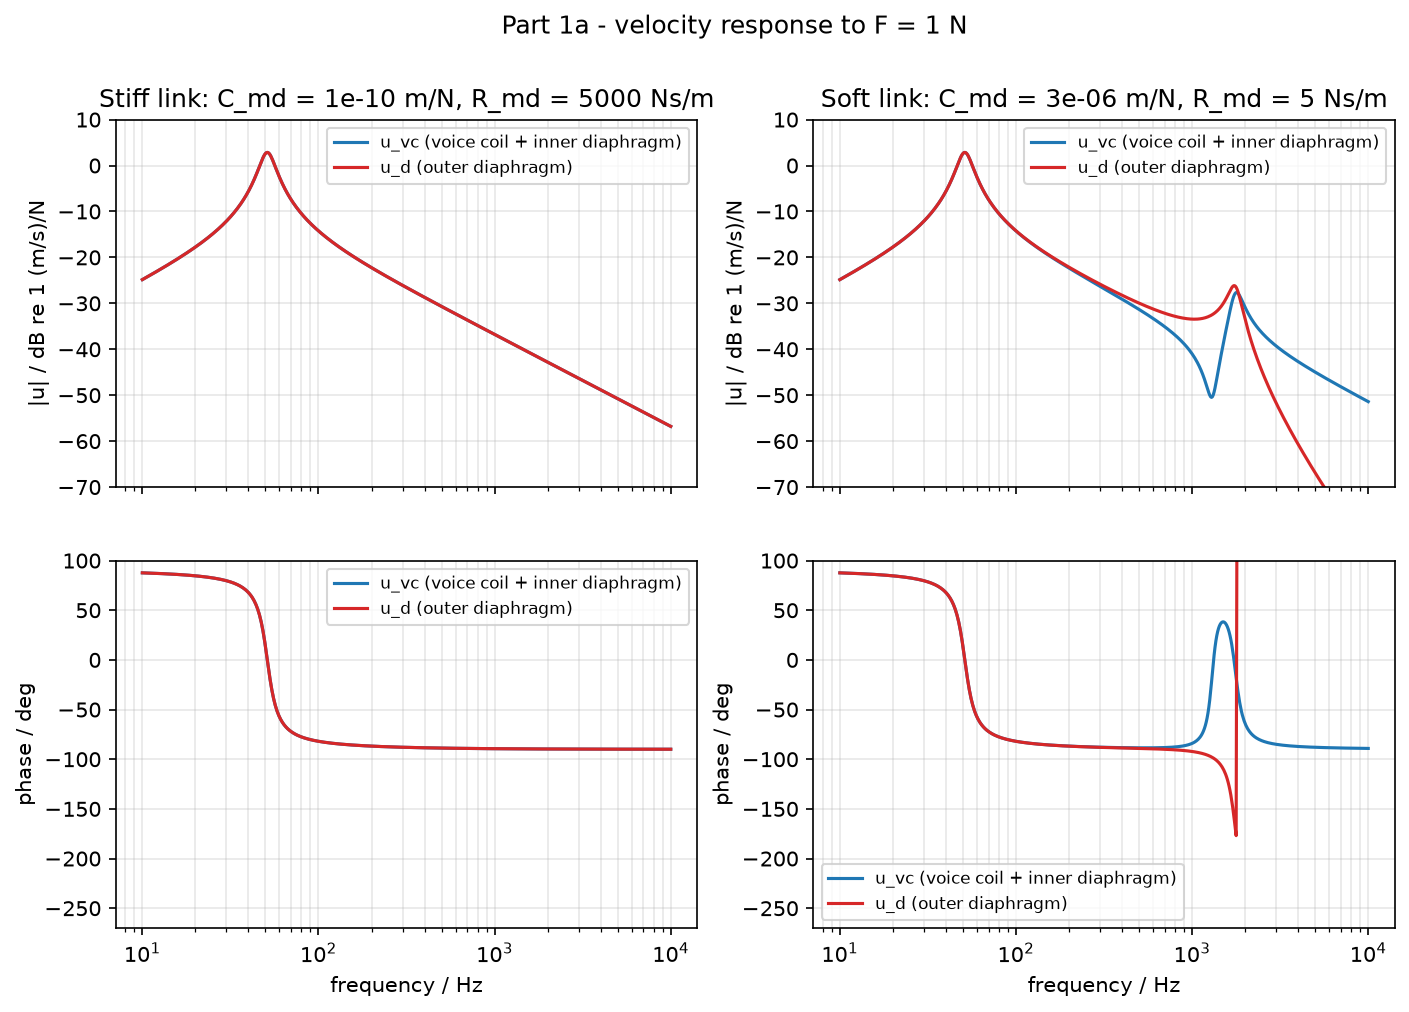
\includegraphics[width=\linewidth]{part1a_velocities}
\caption{Part 1a: velocity of the coil/inner diaphragm $u_{vc}$ and of the outer diaphragm $u_d$ per newton of
force ($F = \SI{1}{\newton}$ AC), magnitude and phase, stiff link (left) and soft link (right), \SIrange{10}{10000}{\hertz}.}
\label{fig:p1a}
\end{figure}

\begin{figure}[!htb]\centering
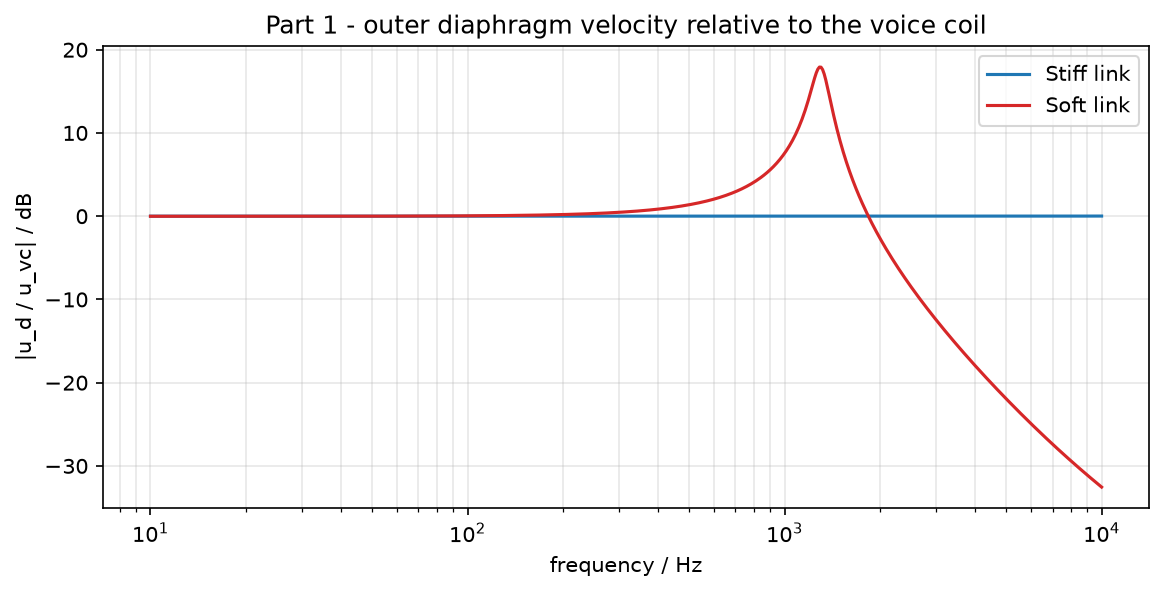
\includegraphics[width=0.8\linewidth]{part1_velocity_ratio}
\caption{Part 1a: ratio $u_d/u_{vc}$ for the two links --- unity for the stiff link, the mechanical crossover for the soft link.}
\label{fig:p1ratio}
\end{figure}

\FloatBarrier
\paragraph{b) Mechanical input impedance $Z_M = F/u_{vc}$ (Fig.~\ref{fig:p1b}).}
\begin{table}[H]\centering\small
\begin{tabular}{@{}llll@{}}\toprule
Case & Feature & $f$ & $Z_M$ [\si{\newton\second\per\metre}] \\ \midrule
both & compliance asymptote & \SI{10}{\hertz} & $0.72 - j17.4$ ($\approx 1/(\omega C_{tot}) = 18.1$) \\
both & resonance (minimum) & \SI{51.3}{\hertz} & $0.720 = R_{tot}$, phase \SI{0}{\degree} \\
Stiff & mass asymptote & \SI{10}{\kilo\hertz} & $0.74 + j692$ ($=\omega M_{tot}$, \SI{11}{\gram}) \\
Soft & anti-resonance (maximum) & \SI{1288}{\hertz} & 334 \\
Soft & second resonance (minimum) & \SI{1799}{\hertz} & 24.1 \\
Soft & mass asymptote & \SI{10}{\kilo\hertz} & $5.7 + j372$ ($=\omega M_{mvc}$, only the \SI{6}{\gram} coil) \\
\bottomrule\end{tabular}
\caption{Part 1b extracted numbers.}
\end{table}

The impedance is the mirror image of $u_{vc}$ (with a \SI{1}{\ampere} source it is literally $1/V(u_{vc})$). Below
resonance the suspension dominates: $|Z|\propto 1/f$ with phase \SI{-90}{\degree}, the \emph{compliance line}. At
resonance the reactances cancel and the floor is the pure damping $R_{tot} = \SI{0.72}{\newton\second\per\metre}$ at
phase \SI{0}{\degree}. Above resonance the mass dominates: $|Z|\propto f$ with phase $+\SI{90}{\degree}$, the
\emph{mass line}. For the stiff link the mass line follows \SI{11}{\gram} all the way to \SI{10}{\kilo\hertz}. For the
soft link it follows \SI{11}{\gram} up to about \SI{1}{\kilo\hertz}, then the absorber produces a \emph{maximum}
(anti-resonance, \SI{334}{\newton\second\per\metre}: the outer diaphragm pumps force back into the coil), then a
\emph{minimum} at \SI{1.8}{\kilo\hertz} (anti-phase resonance), and finally the line continues at only \SI{6}{\gram}
because the outer diaphragm has fallen off. The residual real part of \SI{5.7}{\newton\second\per\metre} at
\SI{10}{\kilo\hertz} is the power still dissipated in $R_{md}$ by the relative motion of the two masses.

\begin{figure}[!htb]\centering
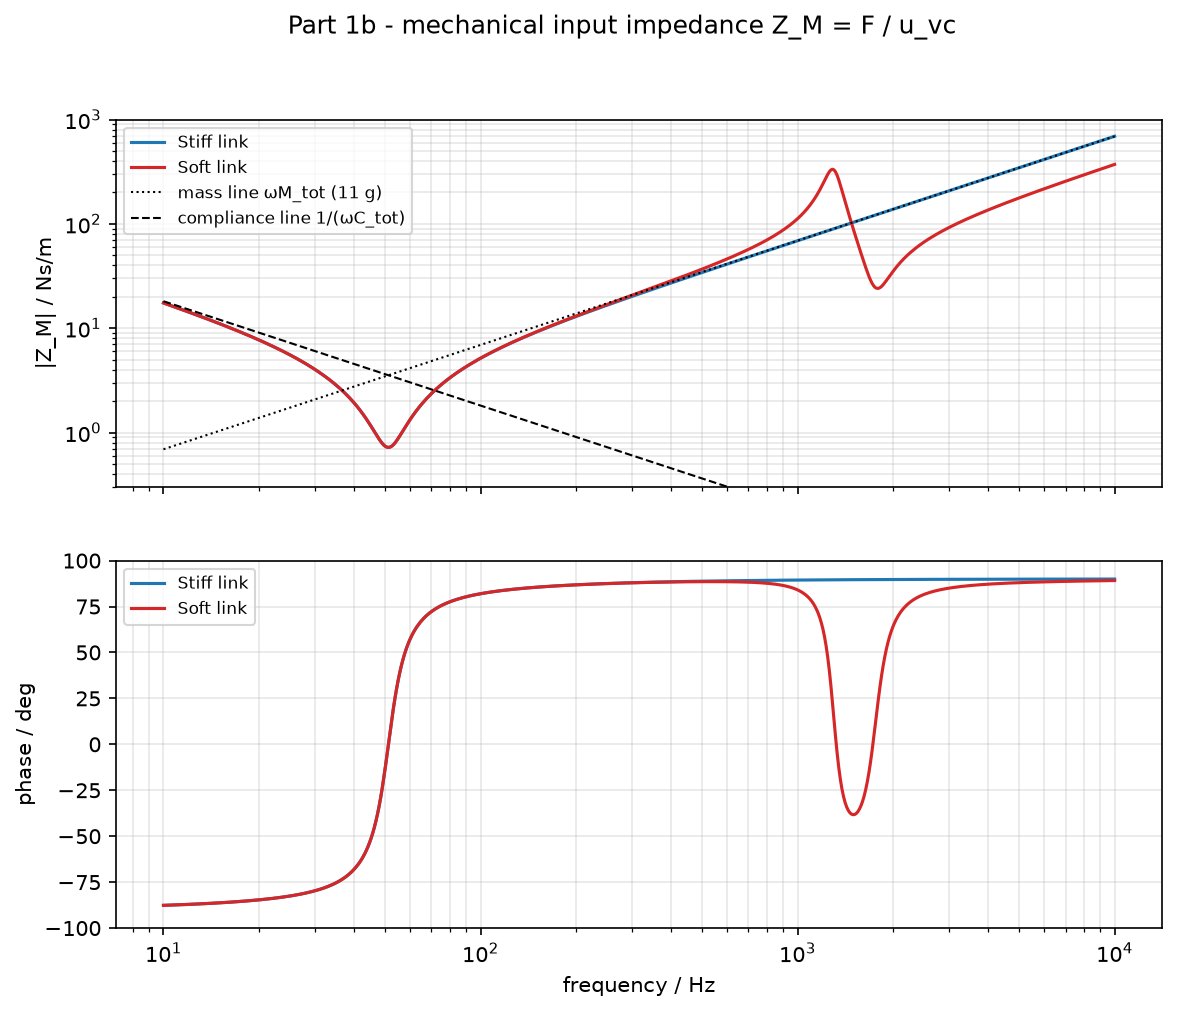
\includegraphics[width=0.85\linewidth]{part1b_impedance}
\caption{Part 1b: mechanical input impedance seen by the force, magnitude and phase, stiff and soft link.}
\label{fig:p1b}
\end{figure}

\FloatBarrier
\paragraph{Modelling choices and validity.} No acoustic load (as instructed), so all damping is the three mechanical
dampers and the response is that of an ideal lumped two-mass system; a real cone would add break-up modes above a
few kilohertz. The frequencies are read from a 200-points-per-decade sweep, accurate to about \SI{0.5}{\percent}.


%% ======================================================================
\FloatBarrier
\section{Part 2 --- Acoustic system: car silencer}
\subsection{Model}
Elements 1, 3, 5, 7 are narrow tubes (radius \SI{2}{\milli\metre}); each is an acoustic mass
$M_A = \rho l/S$ in series with the given loss $R_A = \SI{25e3}{\pascal\second\per\cubic\metre}$. Elements
2, 4, 6 are expansion chambers; each is a compliance $C_A = V/(\rho c^2)$ from its node to the reference
pressure (ground). The result is a ladder network (a low-pass filter), driven either by a pressure source
(voltage) or a volume-velocity source (current).

\begin{table}[H]\centering\small
\begin{tabular}{@{}lllllll@{}}\toprule
Element & $r$ [mm] & $l$ [mm] & $S$ or $V$ & $M_A$ [\si{\kilo\gram\per\metre\tothe{4}}] & $C_A$ [\si{\metre\tothe{5}\per\newton}] & $R_A$ \\ \midrule
1 tube    & 2  & 25  & \SI{1.257e-5}{\square\metre} & 2348 & --- & \SI{25e3}{} \\
2 chamber & 10 & 50  & \SI{15.7}{\cubic\centi\metre} & --- & \num{1.125e-10} & --- \\
3 tube    & 2  & 80  & \SI{1.257e-5}{\square\metre} & 7512 & --- & \SI{25e3}{} \\
4 chamber & 20 & 80  & \SI{100.5}{\cubic\centi\metre} & --- & \num{7.200e-10} & --- \\
5 tube    & 2  & 100 & \SI{1.257e-5}{\square\metre} & 9390 & --- & \SI{25e3}{} \\
6 chamber & 15 & 60  & \SI{42.4}{\cubic\centi\metre} & --- & \num{3.037e-10} & --- \\
7 tube    & 2  & 40  & \SI{1.257e-5}{\square\metre} & 3756 & --- & \SI{25e3}{} \\
\bottomrule\end{tabular}
\caption{Silencer element values (effective lengths as given in the lab).}
\end{table}

\begin{figure}[H]\centering
\begin{circuitikz}[american,scale=0.8,every node/.style={transform shape}]
\draw (0,0) node[ground]{} to[V, l=$p$ or $U$] (0,2.5)
  to[R, l=$R_{A1}$] (2,2.5) to[L, l=$M_{A1}$] (4,2.5) node[circ]{} node[above]{$p_2$}
  to[R, l=$R_{A3}$] (6,2.5) to[L, l=$M_{A3}$] (8,2.5) node[circ]{} node[above]{$p_4$}
  to[R, l=$R_{A5}$] (10,2.5) to[L, l=$M_{A5}$] (12,2.5) node[circ]{} node[above]{$p_6$}
  to[R, l=$R_{A7}$] (14,2.5) to[L, l=$M_{A7}$] (16,2.5) node[circ]{} node[above]{$p_{out}$};
\draw (4,2.5) to[C, l_=$C_{A2}$] (4,0) node[ground]{};
\draw (8,2.5) to[C, l_=$C_{A4}$] (8,0) node[ground]{};
\draw (12,2.5) to[C, l_=$C_{A6}$] (12,0) node[ground]{};
\draw (16,2.5) to[generic, l_=$\Zrad$] (16,0) node[ground]{};
\end{circuitikz}
\caption{Silencer ladder. For a)--c) the outlet is an ideal open end ($\Zrad = 0$, $p_{out} = 0$); for d)--e)
the tube-end radiation network is inserted.}
\end{figure}

\paragraph{Radiation impedance at the outlet (d, e).} For an unflanged tube end of radius $a$ (piston in a
long tube, Lecture 3 \S8b) the fitted network is $\Zrad = \jw M_{A1} \,\|\, [R_{A2} + (R_{A1}\,\|\,C_{A1})]$
with $M_{A1} = 0.6133\rho/(\pi a)$, $C_{A1} = 0.55\pi^2 a^3/(\rho c^2)$, $R_{A1} = 0.5045\rho c/(\pi a^2)$,
$R_{A2} = \rho c/(\pi a^2)$. With $a = \SI{2}{\milli\metre}$: $M_{A1} = \SI{115.2}{\kilo\gram\per\metre\tothe{4}}$,
$C_{A1} = \SI{3.11e-13}{\metre\tothe{5}\per\newton}$, $R_{A1} = \SI{1.63e7}{}$, $R_{A2} = \SI{3.23e7}{\pascal\second\per\cubic\metre}$.
Because the given pipe lengths are already \emph{effective} lengths, the end correction $0.6133a = \SI{1.23}{\milli\metre}$
is subtracted from pipe 7 when the radiation mass is present, so it is not counted twice.
Over the whole band $ka \le 0.037$, so the radiation load is essentially the mass $M_{A1}$ and the near-field
pressure at the opening is $p_{out} \approx \jw M_{A1}U_{out}$.


\subsection{Results and discussion}
Hand estimates of the natural frequencies from single mass--compliance pairs are only a rough guide, since the
ladder is a three-degree-of-freedom system whose modes mix neighbouring elements. The most useful estimates take a
chamber with the two tubes on either side of it \emph{in parallel}: $C_{A2}$ with $M_{A1}\|M_{A3}$ gives
\SI{355}{\hertz}, $C_{A4}$ with $M_{A3}\|M_{A5}$ \SI{92}{\hertz}, $C_{A6}$ with $M_{A5}\|M_{A7}$ \SI{176}{\hertz};
the first and last coincide with simulated peaks. All four masses in series (\SI{23006}{\kilo\gram\per\metre\tothe{4}})
against all three compliances in parallel (\SI{1.136e-9}{\metre\tothe{5}\per\newton}) give \SI{31}{\hertz}.

\FloatBarrier
\paragraph{a) Pressure source (Fig.~\ref{fig:p2a}).}
\begin{table}[H]\centering\small
\begin{tabular}{@{}lll@{}}\toprule
Feature & $f$ & $|U_{out}/p_{in}|$ [dB re \SI{1}{\cubic\metre\per\second\per\pascal}] \\ \midrule
10 Hz & --- & \num{-123.0} \\
dip & \SI{42.2}{\hertz} & \num{-132.0} \\
\textbf{peak} & \SI{76.7}{\hertz} & \num{-101.0} \\
dip & \SI{142.9}{\hertz} & \num{-143.9} \\
\textbf{peak} & \SI{179.9}{\hertz} & \num{-112.3} \\
dip & \SI{309.0}{\hertz} & \num{-170.3} \\
\textbf{peak} & \SI{354.8}{\hertz} & \num{-149.6} \\
1 kHz & --- & \num{-253.9} \\
\bottomrule\end{tabular}
\caption{Part 2a: output volume velocity of pipe 7 for a \SI{1}{\pascal} pressure source at the inlet.}
\end{table}
The output is $U_{out} = (p_{in}/Z_{in})\cdot(U_{out}/U_{in})$, so with a pressure source the low-frequency level is
set by the \emph{input impedance of the whole ladder} (Fig.~\ref{fig:p2zin}). Below about \SI{1}{\hertz} that would be
the four series losses $\sum R_A = \SI{e5}{\pascal\second\per\cubic\metre}$ (\SI{-100}{\decibel}), but already at
\SI{10}{\hertz} the series air masses dominate: $\omega\sum M_A = 2\pi\cdot 10\cdot 23006 = \num{1.45e6} \gg \num{e5}$,
hence $|Z_{in}|\approx\num{1.5e6}$ and \SI{-123}{\decibel}. The three peaks (76.7, 179.9, \SI{354.8}{\hertz}) are the
\emph{minima} of $Z_{in}$, i.e.\ the series resonances: with the inlet held at a fixed pressure the natural frequencies
are those of the ladder with a short-circuited ($p = 0$) inlet. The dips are where $U_{out}$ passes through zero between
two poles, close to the $Z_{in}$ maxima (47, 176, \SI{190}{\hertz}) and to the $M_{A1}$--$C_{A2}$ pair
(\SI{310}{\hertz}). Above the last resonance the response falls at about \SI{18}{\decibel} per octave per chamber section
(a ladder of three L--C low-pass sections), from \SI{-150}{\decibel} at \SI{355}{\hertz} to \SI{-254}{\decibel} at
\SI{1}{\kilo\hertz}. The losses $R_A$ only round off the peaks: at \SI{100}{\hertz} $\omega M_{A3} = \num{4.7e6}\gg\num{2.5e4}$,
so the Q-factors are in the hundreds and the peaks are very sharp.

\begin{figure}[!htb]\centering
\begin{subfigure}{0.49\linewidth}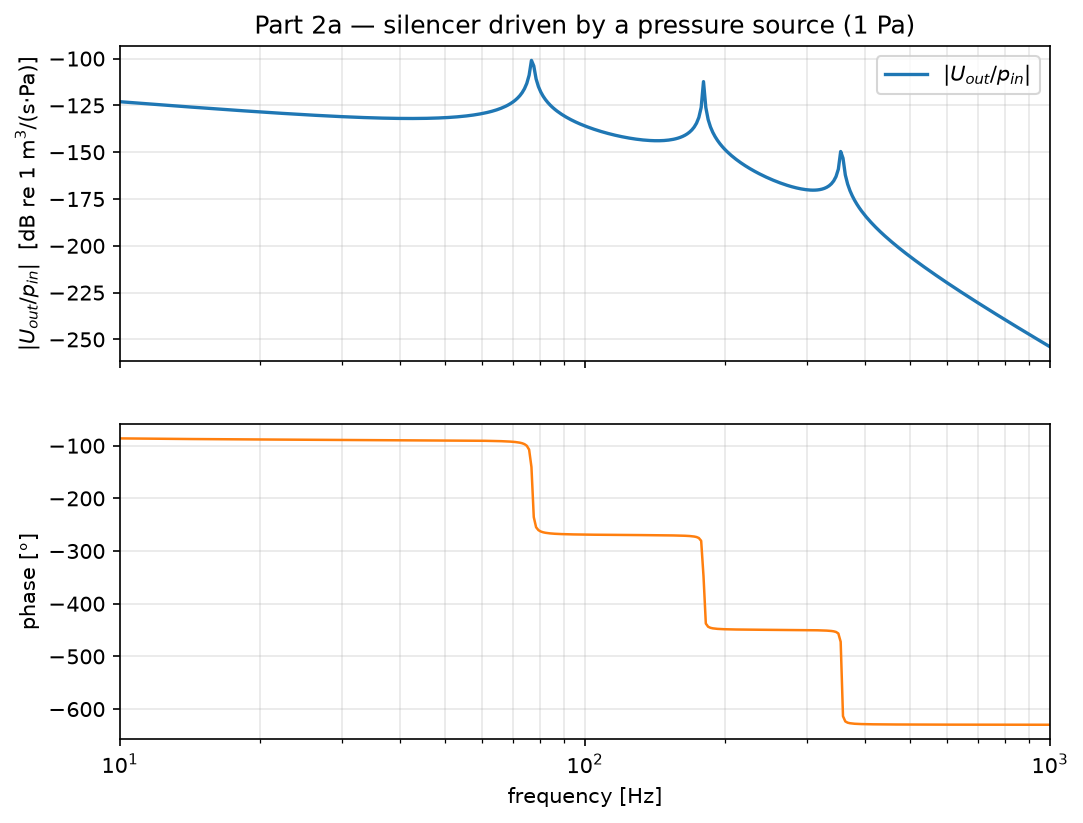
\includegraphics[width=\linewidth]{part2a_pressure_source_Uout}\caption{pressure source, \SI{1}{\pascal}}\label{fig:p2a}\end{subfigure}
\begin{subfigure}{0.49\linewidth}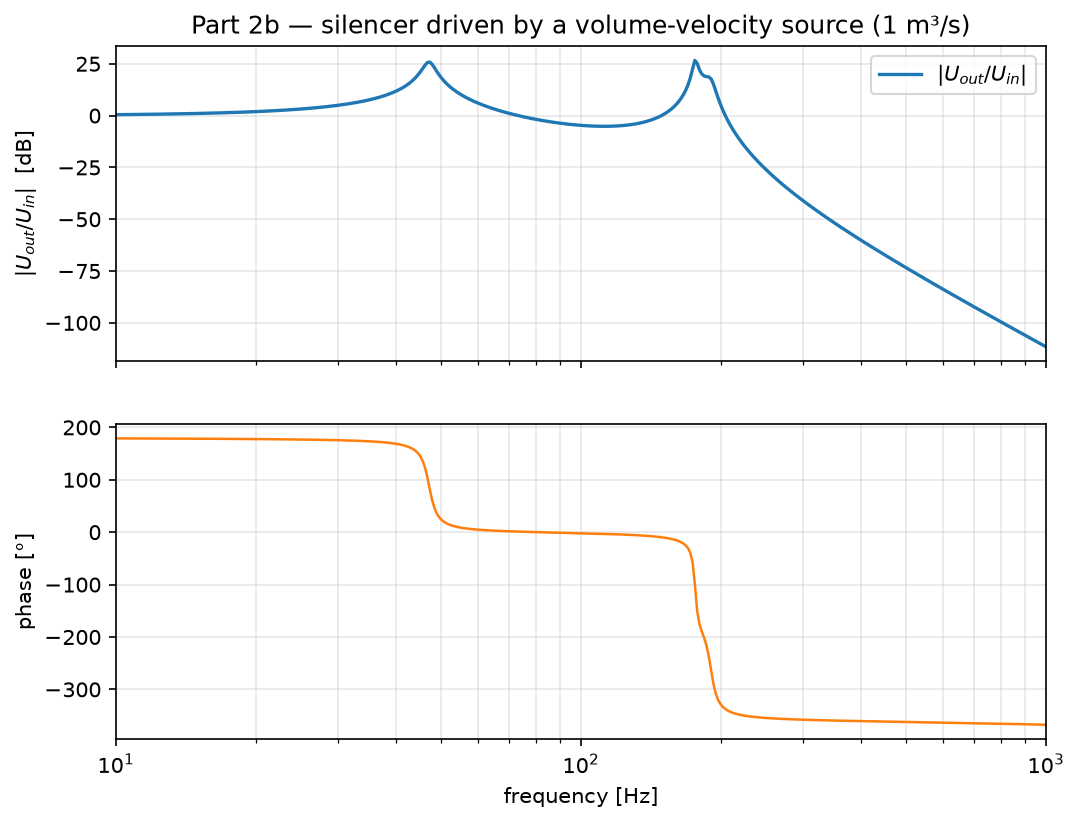
\includegraphics[width=\linewidth]{part2b_volume_velocity_source_Uout}\caption{volume-velocity source, \SI{1}{\cubic\metre\per\second}}\label{fig:p2b}\end{subfigure}
\caption{Part 2a/b: volume velocity in the exit pipe, $|I(V_{s7})|$, magnitude and phase, \SIrange{10}{1000}{\hertz}.}
\end{figure}

\FloatBarrier
\paragraph{b) Volume-velocity source (Fig.~\ref{fig:p2b}) and the difference to a).}
\begin{table}[H]\centering\small
\begin{tabular}{@{}lll@{}}\toprule
Feature & $f$ & $|U_{out}/U_{in}|$ [dB] \\ \midrule
10 Hz & --- & $+0.44$ ($\to 0$ as $f\to 0$) \\
\textbf{peak} & \SI{47.3}{\hertz} & $+25.8$ \\
dip & \SI{112.2}{\hertz} & $-5.2$ \\
\textbf{peak} & \SI{175.8}{\hertz} & $+26.6$ (shoulder at \SI{190}{\hertz}) \\
1 kHz & --- & $-111.5$ \\
\bottomrule\end{tabular}
\caption{Part 2b: transfer $U_{out}/U_{in}$ for the volume-velocity source.}
\end{table}
Transmission loss $\mathrm{TL} = -20\log|U_{out}/U_{in}|$: \SI{-1.9}{\decibel} at \SI{20}{\hertz}, \SI{-18.2}{\decibel}
at \SI{50}{\hertz}, $+4.7$ at 100, $-0.2$ at 150, $-5.5$ at 200, $+40.6$ at 300, $+73.5$ at 500, $+92.2$ at 700 and
$+\SI{111.5}{\decibel}$ at \SI{1}{\kilo\hertz}.

With an ideal volume-velocity source the flow is forced into the inlet whatever pressure it takes. At low frequency the
chambers cannot store flow ($1/(\omega C_A)$ is huge), so everything that goes in comes out: \SI{0}{\decibel}, independent
of the series masses and losses. The transfer $U_{out}/U_{in}$ is a property of the network alone; the source only
decides which natural frequencies are excited. A volume-velocity source is an \emph{open circuit} at the inlet, so the
peaks sit at the open-inlet natural frequencies, the \emph{maxima} of $Z_{in}$ (47.3 and 175.8/\SI{190}{\hertz}) ---
exactly where the pressure-source response has its dips --- while the pressure-source peaks ($Z_{in}$ minima) do not
appear at all (overlay in Fig.~\ref{fig:p2ab}). At those frequencies the ladder resonates and the silencer
\emph{amplifies} the flow by \SI{26}{\decibel}. A real engine exhaust is somewhere between the two ideal sources
(finite source impedance), which is why a silencer design has to know its source impedance. Above \SI{200}{\hertz}
the chambers shunt the flow and the mass of the following pipe blocks it; the roll-off is the same \SI{18}{\decibel}
per octave per section, reaching \SI{111}{\decibel} of transmission loss at \SI{1}{\kilo\hertz}. Only two clear peaks
appear instead of three because the third open-inlet mode at \SI{190}{\hertz} sits right next to \SI{176}{\hertz}
and only shows as a shoulder.

\begin{figure}[!htb]\centering
\begin{subfigure}{0.49\linewidth}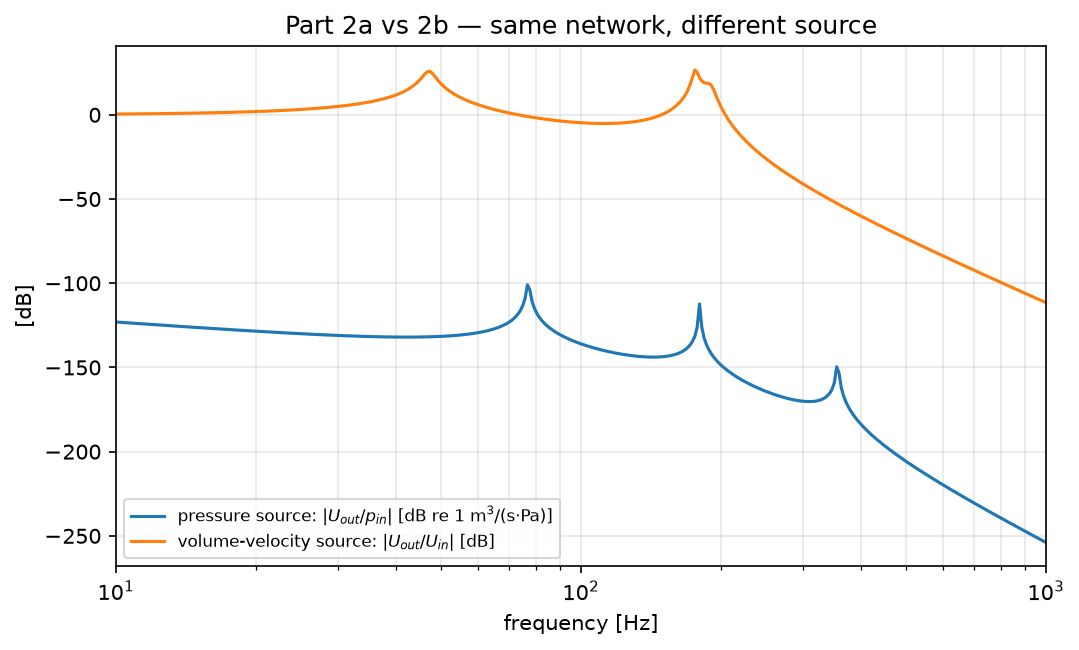
\includegraphics[width=\linewidth]{part2ab_source_comparison}\caption{$U_{out}$ for both sources, normalised}\label{fig:p2ab}\end{subfigure}
\begin{subfigure}{0.49\linewidth}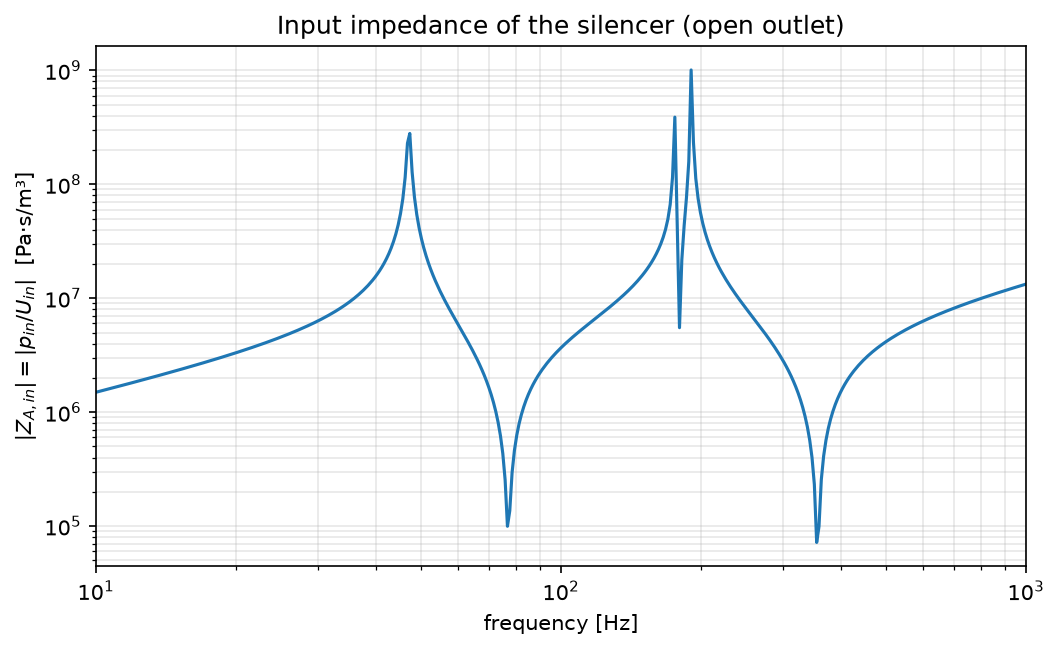
\includegraphics[width=\linewidth]{part2_input_impedance}\caption{input impedance $Z_{in} = p_{in}/U_{in}$ of the ladder}\label{fig:p2zin}\end{subfigure}
\caption{Part 2: why the two sources excite different resonances --- the pressure source peaks at the minima of
$Z_{in}$, the volume-velocity source at its maxima.}
\end{figure}

\FloatBarrier
\paragraph{c) Volume velocity in each pipe, volume-velocity source (Fig.~\ref{fig:p2c}).}
\begin{table}[H]\centering\small
\begin{tabular}{@{}lll@{}}\toprule
Pipe & Level at \SI{1}{\kilo\hertz} & Peaks / dips \\ \midrule
1 & \SI{0}{\decibel} everywhere & (it \emph{is} the source current) \\
3 & \SI{-30.2}{\decibel} & $+8.7$ dB at 47 Hz, $+19.9$ at 176 Hz, $+22.0$ at 191 Hz; dip \SI{-22}{\decibel} at \SI{51}{\hertz} \\
5 & \SI{-78.7}{\decibel} & $+24.9$ at 47 Hz, $+18.5$ at 176 Hz, $+14.2$ at 188 Hz; dip \SI{-39}{\decibel} at \SI{150}{\hertz} \\
7 & \SI{-111.5}{\decibel} & $+25.8$ at 47 Hz, $+26.6$ at 176 Hz \\
\bottomrule\end{tabular}
\caption{Part 2c: volume velocity in pipes 1, 3, 5, 7 relative to $U_{in}$.}
\end{table}
$I(V_{s1}) = U_{in}$ by definition, a flat \SI{0}{\decibel} line. Each expansion chamber acts as an acoustic low-pass:
chamber 2 shunts part of $U_1$ so $U_3 < U_1$, chamber 4 takes another bite, chamber 6 the last. At \SI{1}{\kilo\hertz}
the cumulative attenuation is 30, 79 and \SI{112}{\decibel} after one, two and three chambers, i.e.\ each section
contributes 30--\SI{40}{\decibel} there. The dips in $U_3$ (\SI{51}{\hertz}) and $U_5$ (\SI{150}{\hertz}) are
anti-resonances where the downstream part of the ladder presents a very high impedance, so almost no flow enters that
pipe and the chamber before it takes it all; pipe 7 has no dip because nothing follows it. The resonance peaks appear in
every pipe but grow towards the outlet: energy stored in the resonating chambers is released into the pipe after them.

\begin{figure}[!htb]\centering
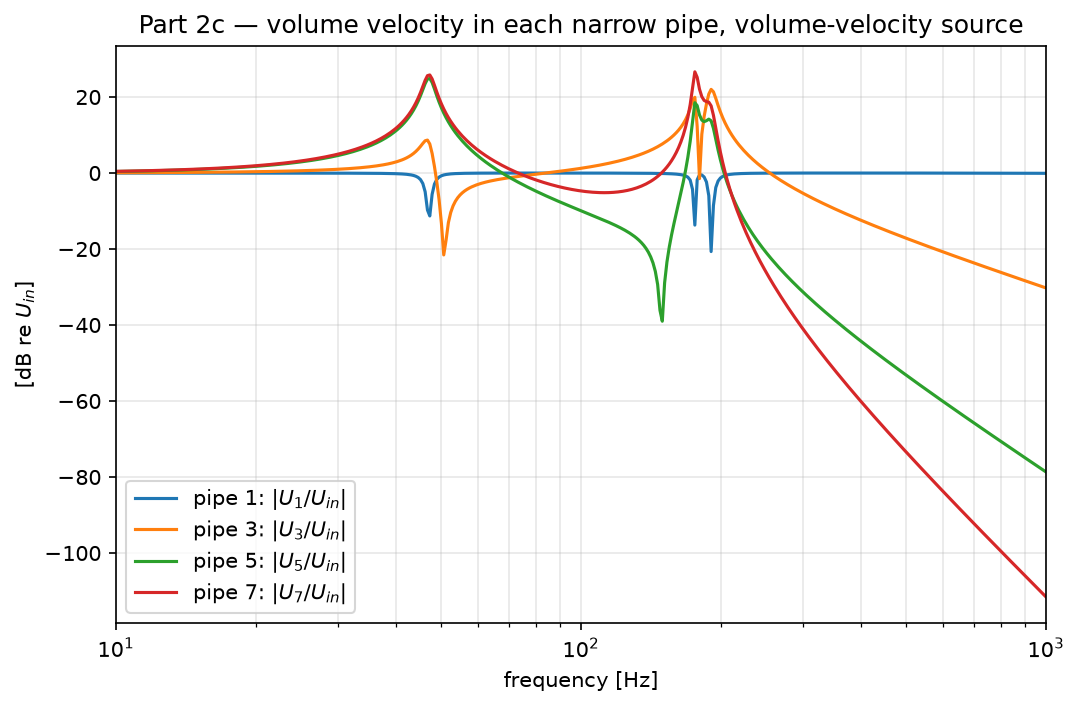
\includegraphics[width=0.75\linewidth]{part2c_pipe_volume_velocities}
\caption{Part 2c: $|I(V_{s1})|$, $|I(V_{s3})|$, $|I(V_{s5})|$, $|I(V_{s7})|$ in dB re $U_{in} = \SI{1}{\cubic\metre\per\second}$.}
\label{fig:p2c}
\end{figure}

\FloatBarrier
\paragraph{d) Near-field pressure at the opening (Fig.~\ref{fig:p2d}).} With the radiation network in place,
$p_{open} = V(p_{out})$: \SI{77.6}{\decibel} re \SI{1}{\pascal} at \SI{10}{\hertz} (\SI{7.6}{\kilo\pascal} per
\si{\cubic\metre\per\second}), \SI{92.5}{\decibel} at \SI{100}{\hertz}, \SI{5.7}{\decibel} at \SI{1}{\kilo\hertz}. The
radiation impedance of the \SI{2}{\milli\metre} tube end is essentially a \emph{pure mass} over the whole band:
$ka = 0.037$ at \SI{1}{\kilo\hertz}, $|\Zrad| = \SI{7.24e5}{\pascal\second\per\cubic\metre}$ with a real part of only
\num{1.08e4} (\SI{1.5}{\percent}); the resistive $R_{A2} = \num{3.2e7}$ is only reached near $ka = 1$ at \SI{27}{\kilo\hertz}.
Consequently $p_{open}\approx \jw M_{A1}U_{out}$: the dashed curve $\omega M_{A1}|U_{out}|$ lies on top of the simulated
pressure, and the pressure curve is simply the $U_{out}$ curve of b) tilted by $+\SI{6}{\decibel}$ per octave, with the
same peaks at 47 and \SI{176}{\hertz}. Inserting the radiation load changes $U_{out}$ by less than \SI{0.01}{\decibel}:
$|\Zrad|\le\num{7e5}$ against a pipe-7 impedance $\omega M_{A7}$ of \num{2.3e5} at \SI{10}{\hertz} and \num{2.3e7} at
\SI{1}{\kilo\hertz}. The silencer does not ``see'' the outside air; the ideal open end used in a)--c) is an excellent
approximation.

\begin{figure}[!htb]\centering
\begin{subfigure}{0.49\linewidth}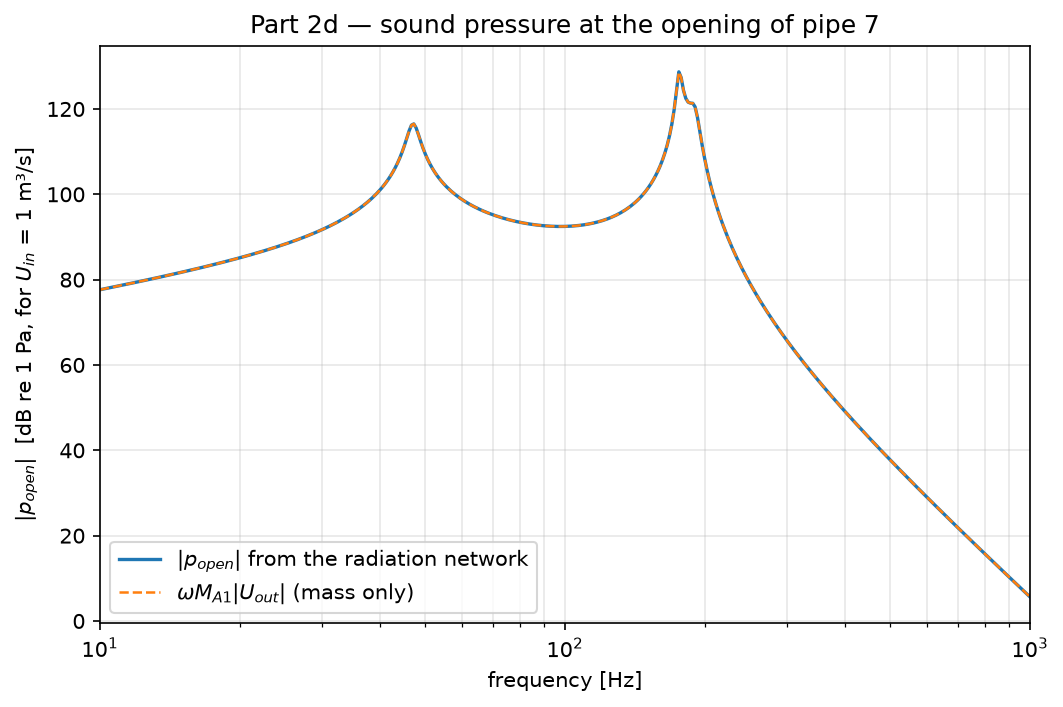
\includegraphics[width=\linewidth]{part2d_near_field_pressure}\caption{near field, $p_{open} = V(p_{out})$}\label{fig:p2d}\end{subfigure}
\begin{subfigure}{0.49\linewidth}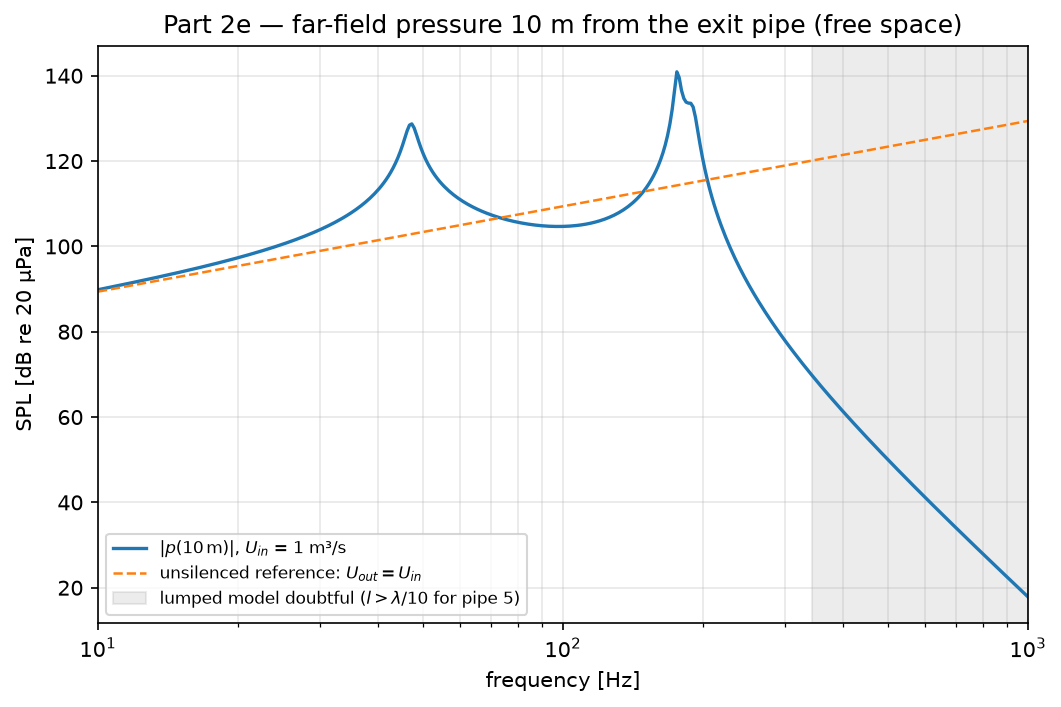
\includegraphics[width=\linewidth]{part2e_pressure_10m}\caption{far field, \SI{10}{\metre}, free space}\label{fig:p2e}\end{subfigure}
\caption{Part 2d/e: sound pressure at the exit and at \SI{10}{\metre} for $U_{in} = \SI{1}{\cubic\metre\per\second}$ (a
realistic \SI{e-3}{\cubic\metre\per\second} is \SI{60}{\decibel} lower). The grey band marks where the lumped model is
no longer valid.}
\end{figure}

\FloatBarrier
\paragraph{e) Pressure at \SI{10}{\metre} (Fig.~\ref{fig:p2e}) and validity.} The pipe end radiates into free space
($4\pi$) as a point source: $p(r) = \jw\rho U_{out}e^{-jkr}/(4\pi r)$, so $|p| = \rho f|U_{out}|/(2r)$, computed from
$I(V_{s7})$ of the radiation sheet.
\begin{table}[H]\centering\small
\begin{tabular}{@{}lll@{}}\toprule
$f$ & SPL with silencer [dB re \SI{20}{\micro\pascal}] & unsilenced ($U_{out} = U_{in}$) \\ \midrule
\SI{20}{\hertz} & 97.3 & 95.4 \\
\SI{50}{\hertz} & 121.6 & 103.4 \\
\SI{100}{\hertz} & 104.7 & 109.4 \\
\SI{200}{\hertz} & 120.9 & 115.4 \\
\SI{500}{\hertz} & 49.9 & 123.4 \\
\SI{1}{\kilo\hertz} & 17.9 & 129.4 \\
\bottomrule\end{tabular}
\caption{Part 2e: sound pressure level at \SI{10}{\metre} for $U_{in} = \SI{1}{\cubic\metre\per\second}$.}
\end{table}
The far-field pressure of a monopole rises \SI{6}{\decibel} per octave for constant $U$ (the dashed reference), so the
radiated SPL is the $U_{out}$ transfer of b) plus that tilt. The silencer helps only above about \SI{230}{\hertz}
(roughly \SI{75}{\decibel} at \SI{500}{\hertz}, \SI{110}{\decibel} at \SI{1}{\kilo\hertz}) and \emph{hurts} by up to
\SI{18}{\decibel} at its two resonances when driven by an ideal volume-velocity source.

\emph{Validity at higher frequencies.} Lumped elements require $l < \lambda/10$. Pipe 5 (\SI{100}{\milli\metre}) meets
this only below \SI{344}{\hertz}, pipe 3 and chamber 4 (\SI{80}{\milli\metre}) below \SI{430}{\hertz}, chamber 6 below
\SI{573}{\hertz}, chamber 2 below \SI{688}{\hertz}, pipe 7 below \SI{860}{\hertz}. Above roughly 350--\SI{450}{\hertz} the
pipes and chambers must be treated as transmission lines (ABCD two-ports, Lecture~3 \S4); the smooth lumped roll-off then
becomes a sequence of pass and stop bands (the first half-wave resonance of the \SI{100}{\milli\metre} pipe is
$c/2l = \SI{1.7}{\kilo\hertz}$, of the \SI{80}{\milli\metre} chamber \SI{2.15}{\kilo\hertz}). The \SI{111}{\decibel} of
transmission loss at \SI{1}{\kilo\hertz} is therefore not to be trusted. The plane-wave assumption across the chamber
radius holds ($ka = 1$ at \SI{2.7}{\kilo\hertz} for the \SI{20}{\milli\metre} chamber); the point-source assumption for
the \SI{2}{\milli\metre} exit is excellent ($ka\ll 1$ to tens of kilohertz) and $r = \SI{10}{\metre}\gg\lambda$ except at
the lowest frequencies. Free-space radiation ignores the car body and the road (a tailpipe near the ground sees a
half-space, $+\SI{6}{\decibel}$, plus reflections); the constant loss $R_A$ is crude, since viscous losses in a
\SI{2}{\milli\metre} pipe grow with $\sqrt f$; the walls are assumed rigid, and hot exhaust gas has a different $\rho$
and $c$ than the \SI{20}{\celsius} air assumed here.


%% ======================================================================
\FloatBarrier
\section{Part 3 --- Coupled mechanical--acoustic system}
\subsection{Model}
Each diaphragm now radiates from both sides into an infinite baffle. A piston of area $S$ sees, per side,
the baffled-piston radiation impedance (Lecture 3 \S8b)
\[
\Zrad(a) = \jw M_{A1}\,\|\,\big[R_{A2} + (R_{A1}\,\|\,C_{A1})\big],
\]
\[
M_{A1} = \frac{8\rho}{3\pi^2 a},\qquad R_{A1} = 0.441\frac{\rho c}{\pi a^2},\qquad R_{A2} = \frac{\rho c}{\pi a^2},\qquad
C_{A1} = 5.94\frac{a^3}{\rho c^2},
\]
and both sides together give $2\Zrad$. The coupling to the mobility circuit uses $U = S u$ and $f = S p$: a
VCCS with gain $S$ injects the volume velocity into the acoustic sub-network, and a second VCCS with gain $S$
draws the reaction force $S p$ from the velocity node. Seen from the mechanical side this is the load
$Z_{M,A} = S^2\cdot 2\Zrad$ (an admittance $S^2\cdot 2\Zrad$ in the mobility circuit).

\begin{table}[H]\centering\small
\begin{tabular}{@{}lcccccccc@{}}\toprule
Diaphragm & $S$ & $a$ & $M_{A1}$ & $R_{A1}$ & $R_{A2}$ & $C_{A1}$ & $2S^2M_{A1}$ & $2S^2R_{A2}$ \\
 & [\si{\square\centi\metre}] & [mm] & [\si{\kilo\gram\per\metre\tothe{4}}] & \multicolumn{2}{c}{[\si{\pascal\second\per\cubic\metre}]} & [\si{\metre\tothe{5}\per\newton}] & [g] & [\si{\newton\second\per\metre}] \\ \midrule
inner & 60 & 43.7 & 7.295 & 29835 & 67653 & \num{3.55e-9} & 0.525 & 4.87 \\
outer & 210 & 81.8 & 3.900 & 8524 & 19330 & \num{2.33e-8} & 3.44 & 17.05 \\
\bottomrule\end{tabular}
\caption{Radiation-impedance constants per side, and the resulting added mass (low $ka$) and added
resistance (high $ka$) for both sides. $ka = 1$ at \SI{1253}{\hertz} (inner) and \SI{670}{\hertz} (outer).}
\end{table}

\begin{figure}[H]\centering
\begin{circuitikz}[american,scale=0.85,every node/.style={transform shape}]
% mechanical node
\draw (0,0) node[ground]{} to[isource, l=$F$] (0,3) -- (1.5,3) node[circ]{} node[above]{$u$};
\draw (1.5,3) to[generic, l_=$Y_M$ (Part 1)] (1.5,0) node[ground]{};
% force sink
\draw (3.5,3) to[cI, l_=$S\,p$, invert] (3.5,0) node[ground]{};
\draw (1.5,3) -- (3.5,3);
% acoustic side
\draw (6.5,0) node[ground]{} to[cI, l=$S\,u$] (6.5,3) -- (8,3) node[circ]{} node[above]{$p$};
\draw (8,3) to[generic, l_=$2\Zrad$] (8,0) node[ground]{};
\end{circuitikz}
\caption{Coupling block used for each diaphragm in Part 3 (mobility on the left, acoustic impedance analogy
on the right). The left controlled source senses $p$ and draws the reaction force, the right one senses $u$ and injects the volume velocity. The pressure on \emph{one} side of the diaphragm is $p/2$.}
\end{figure}


\subsection{Results and discussion}
\FloatBarrier
\paragraph{Sign check of the coupling.} With the air load the resonance moves \emph{down} (51.3 to \SI{43.7}{\hertz};
hand: $51.2\sqrt{11/(11+0.525+3.44)} = \SI{43.9}{\hertz}$), the peak velocity \emph{drops} (1.389 to
\SI{1.314}{\metre\per\second\per\newton}) and the real part of $Z_M$ at \SI{10}{\kilo\hertz} rises from 0.74 to
\SI{22.8}{\newton\second\per\metre} ($= 0.72 + 4.87 + 17.05 = 22.6$). A wrong polarity of either controlled source would
have raised the peak or made the circuit unstable, so the coupling is a passive load as it must be.

\FloatBarrier
\paragraph{a) Velocities and impedance with and without air (Figs.~\ref{fig:p3a}, \ref{fig:p3z}).}
\begin{table}[H]\centering\small
\begin{tabular}{@{}lllll@{}}\toprule
Case & Feature & Part 1 (no air) & Part 3 (with air) \\ \midrule
Stiff & resonance & \SI{51.3}{\hertz}, 1.389 & \SI{43.7}{\hertz}, 1.314 \\
Stiff & $|Z_M|$ minimum & 0.720 & 0.761 \\
Stiff & $Z_M$ at \SI{10}{\kilo\hertz} & $0.74 + j692$ & $22.8 + j693$ \\
Soft & first resonance & \SI{51.3}{\hertz}, 1.388 & \SI{43.7}{\hertz}, 1.314 \\
Soft & $u_{vc}$ dip / $|Z_M|$ maximum & \SI{1288}{\hertz}, 334 & \SI{1023}{\hertz}, 129 \\
Soft & second resonance ($u_{vc}$ peak, $|Z_M|$ min) & \SI{1799}{\hertz}, 0.0415, 24.1 & \SI{1718}{\hertz}, 0.0264, 37.9 \\
Soft & $u_d$ maximum & \SI{1738}{\hertz}, 0.0493 & \SI{1549}{\hertz}, 0.0257 \\
Soft & $Z_M$ at \SI{10}{\kilo\hertz} & $5.7 + j372$ & $10.6 + j372$ \\
Soft & $u_{vc}/u_d$ at \SI{10}{\kilo\hertz} & 42 & 43 \\
\bottomrule\end{tabular}
\caption{Part 3a: Part 1 versus Part 3. Velocities in \si{\metre\per\second\per\newton}, impedances in \si{\newton\second\per\metre}.}
\end{table}

\emph{Low frequency, $ka\ll1$.} The radiation impedance is almost purely mass-like ($\jw M_{A1}$ dominates the parallel
network): the air adds \SI{0.5}{\gram} on the inner and \SI{3.4}{\gram} on the outer diaphragm to the \SI{11}{\gram}, so
the resonance drops to \SI{43.7}{\hertz} for both links. The radiation resistance there is tiny ($\propto(ka)^2$), so the
peak height is nearly unchanged; the drop from 1.389 to 1.314 is mostly the Q change from the extra mass at fixed $R$.

\emph{Around $ka\approx1$} (\SI{670}{\hertz} outer, \SI{1253}{\hertz} inner) the network turns resistive. For the soft
link the absorber frequency of the outer diaphragm drops from 1288 to \SI{1023}{\hertz} (its mass grew from 5 to
\SI{8.4}{\gram}: $1/(2\pi\sqrt{8.44\,\mathrm{g}\cdot 3\,\mathrm{\mu m/N}}) = \SI{1000}{\hertz}$) and, more importantly,
its \SI{17}{\newton\second\per\metre} of radiation resistance damps the absorber: the $u_{vc}$ dip is \SI{8}{\decibel}
shallower and the anti-resonance in $Z_M$ falls from 334 to \SI{129}{\newton\second\per\metre}. The second resonance is
likewise lower in frequency and about \SI{4}{\decibel} lower in amplitude.

\emph{High frequency, $ka\gg1$.} The load is a pure resistance $\rho c S^2$ per side. Stiff link:
\SI{21.9}{\newton\second\per\metre} in series with the \SI{11}{\gram} mass line, invisible in $|Z_M|$
(\SI{692}{\newton\second\per\metre} reactive) but it is the entire radiated power. Soft link: only the inner diaphragm is
still moving, so only its \SI{4.87}{\newton\second\per\metre} shows up ($10.6 = 5.7 + 4.9$).

\emph{Effect of the radiation impedance in one sentence:} a frequency-dependent load that is extra mass at low frequency
(lowers every resonance) and extra damping at high frequency (flattens the absorber anti-resonance and sets the radiated
power); on the outer diaphragm it is about seven times larger than on the inner one.


\begin{figure}[!htb]\centering
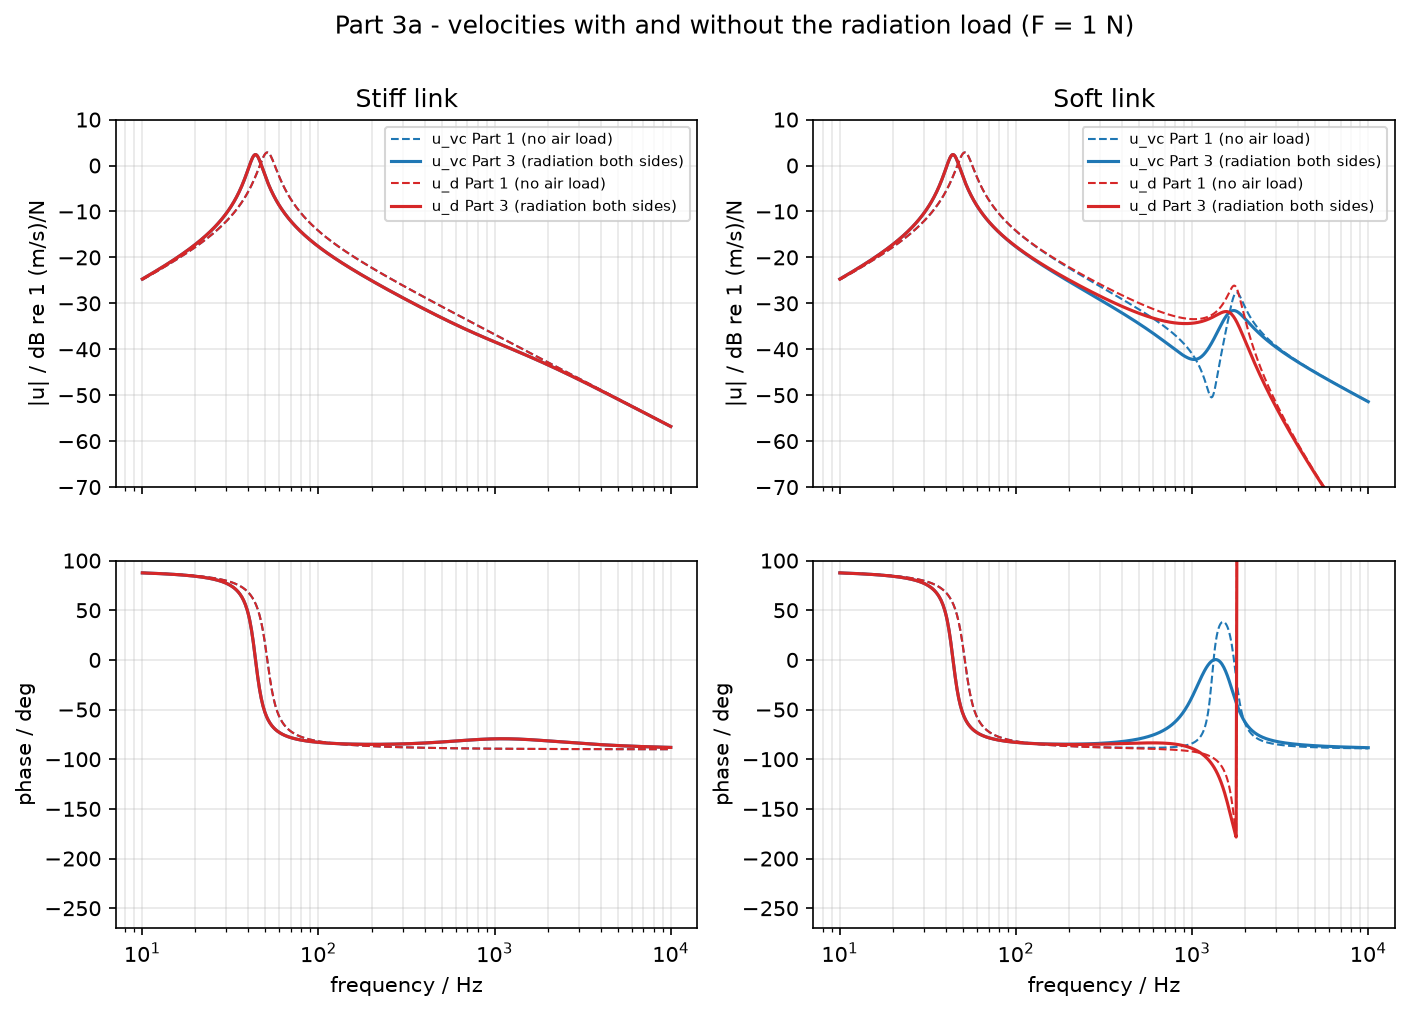
\includegraphics[width=0.92\linewidth]{part3a_velocities}
\caption{Part 3a: $u_{vc}$ and $u_d$ per newton with (solid) and without (dashed, Part 1) radiation loading, stiff and soft link.}
\label{fig:p3a}
\end{figure}

\begin{figure}[!htb]\centering
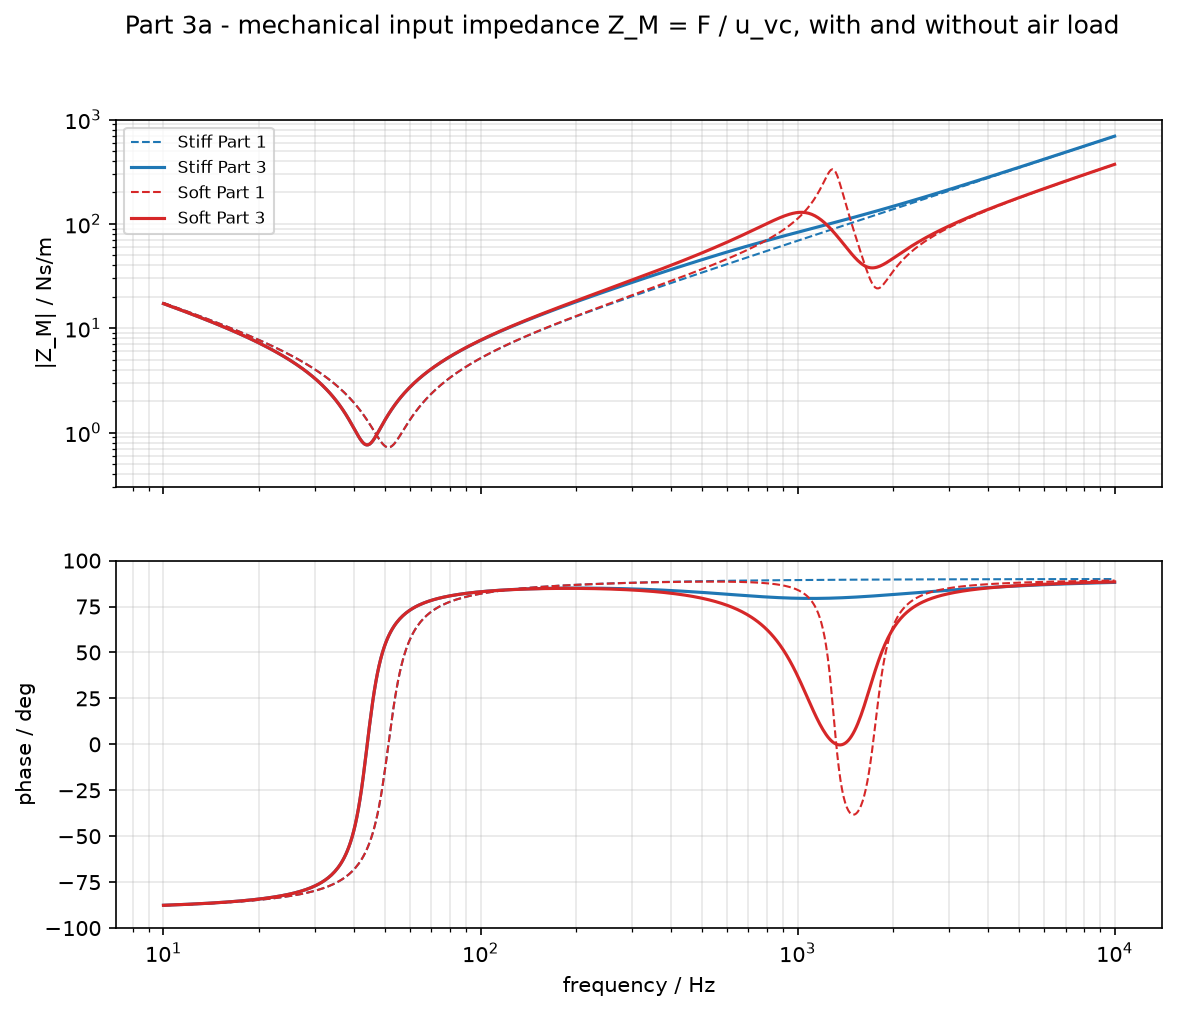
\includegraphics[width=0.72\linewidth]{part3a_impedance}
\caption{Part 3a: mechanical input impedance with (solid) and without (dashed) radiation loading.}
\label{fig:p3z}
\end{figure}

\FloatBarrier
\paragraph{b) Sound pressure (Fig.~\ref{fig:p3b}).} The pressure in front of one face is $V(p_x)/2$, since the $p$ node
carries the sum of both faces. The far-field pressure on axis at \SI{1}{\metre} in the baffle half-space is
$p = \jw\rho(S_iu_{vc} + S_ou_d)/(2\pi\cdot\SI{1}{\metre})$, computed from the node voltages.
\begin{table}[H]\centering\small
\begin{tabular}{@{}lp{5.6cm}p{7.6cm}@{}}\toprule
Case & Quantity & Value [\si{\pascal\per\newton}] \\ \midrule
both & $p_{front}$ inner / outer at the \SI{44}{\hertz} resonance & 15.9 / 29.8 \\
Stiff & $p_{front}$ plateau \SIrange{100}{1000}{\hertz}, inner / outer & $\approx 3$ / 5.6 (10 / \SI{15}{\decibel}) \\
Stiff & $p_{front}$ at \SI{10}{\kilo\hertz}, both & 0.59 \\
Soft & $p_{front}$ inner: 2nd peak / \SI{10}{\kilo\hertz} & 10.0 at \SI{1738}{\hertz} / 1.10 \\
Soft & $p_{front}$ outer: 2nd peak / \SI{10}{\kilo\hertz} & 10.9 at \SI{1567}{\hertz} / 0.03 \\
both & far field peak at \SI{44}{\hertz} & 1.85 \\
Stiff & far field \SIrange{100}{10000}{\hertz} & flat 0.35--0.46 \\
Soft & far field & 0.35 plateau, $+\SI{8}{\decibel}$ hump at \SI{1.6}{\kilo\hertz} (0.87), \SI{-18}{\decibel} dip near \SI{3}{\kilo\hertz} (0.12), 0.18 at \SI{10}{\kilo\hertz} \\
\bottomrule\end{tabular}
\caption{Part 3b extracted numbers.}
\end{table}

\begin{figure}[!htb]\centering
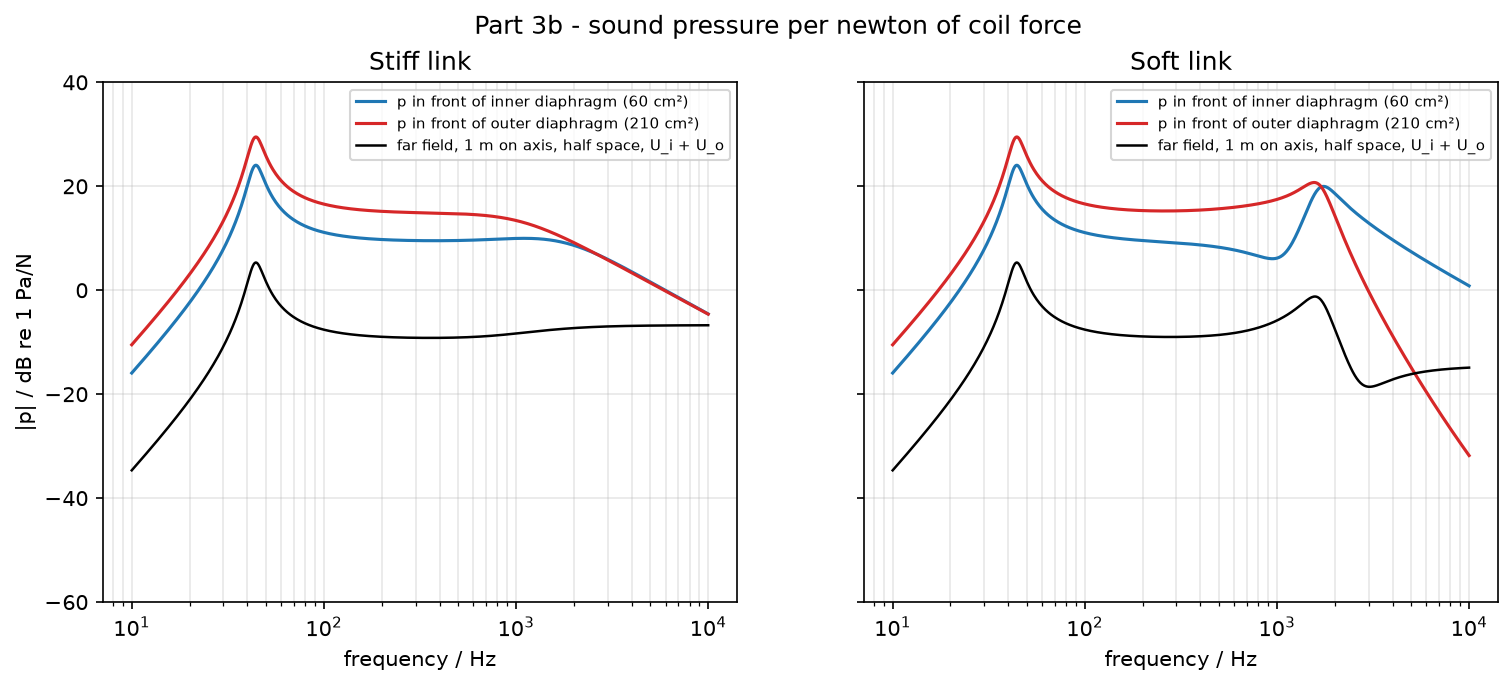
\includegraphics[width=\linewidth]{part3b_pressures}
\caption{Part 3b: pressure in front of each diaphragm and on-axis far-field pressure at \SI{1}{\metre} (half space,
$U_i + U_o$), per newton of coil force.}
\label{fig:p3b}
\end{figure}

The near-field pressure per face is $\Zrad(f)\,S\,u$. Below $ka = 1$ the load is mass-like, so
$p_{front}\approx\omega M_{A1}Su$, which with $u\propto1/f$ gives the flat plateau; the outer face sits \SI{5}{\decibel}
above the inner one because $M_{A1}S\propto a$. Above $ka = 1$ the load is the resistance $\rho c/S$, so
$p_{front}\approx\rho c\,u$ for either face (the same \SI{0.59}{\pascal\per\newton} at \SI{10}{\kilo\hertz} in the stiff
case) and it falls with the velocity. In the far field with constant force, $\omega\rho Su$ is flat in the
mass-controlled region ($\omega\times1/\omega$), the familiar flat loudspeaker response above resonance. The stiff link is
one \SI{11}{\gram} piston, flat to \SI{10}{\kilo\hertz} in this lumped model (a real cone would break up; the model has
no cone modes).

\emph{The dual-diaphragm principle (soft link).} Up to about \SI{1}{\kilo\hertz} the outer cone provides
\SI{78}{\percent} of the volume velocity ($S_o/(S_i+S_o)$). Around \SI{1.6}{\kilo\hertz} the link resonance boosts the
output ($+\SI{8}{\decibel}$ hump, the outer cone resonating on $C_{md}$). Above about \SI{2}{\kilo\hertz} the outer cone
decouples, its velocity falls \SI{12}{\decibel} per octave faster and ends up in anti-phase, so around \SI{3}{\kilo\hertz}
the two partially cancel (dip, Fig.~\ref{fig:p3split}). From about \SI{4}{\kilo\hertz} upward only the inner cone
radiates: \SI{-13}{\decibel} relative to the low-frequency plateau ($=20\log(60/270)$) but \emph{flat}, extending the
bandwidth well beyond where a \SI{210}{\square\centi\metre} cone of \SI{11}{\gram} would have rolled off or broken up.
The design intent is large area for bass efficiency, small light area for treble, and the soft joint is a mechanical
crossover between them.

\begin{figure}[!htb]\centering
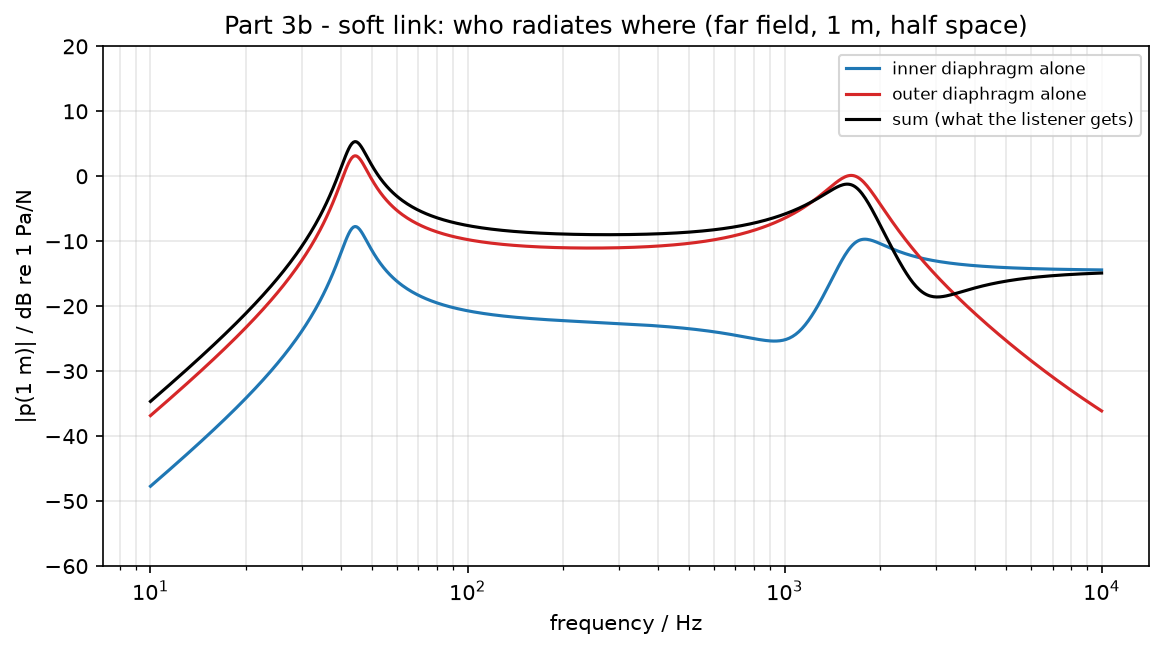
\includegraphics[width=0.8\linewidth]{part3b_farfield_split}
\caption{Part 3b: far-field contribution of each diaphragm and their sum, soft link --- the \SI{3}{\kilo\hertz}
cancellation is where the decoupled outer cone has swung into anti-phase.}
\label{fig:p3split}
\end{figure}

\FloatBarrier
\paragraph{Modelling choices and validity.} As instructed, each diaphragm is loaded as an independent baffled piston
(no mutual radiation impedance between the two, no dipole cancellation of the inner cone even though it sits in the
throat of the outer one) and the total volume velocity is the plain sum $U_i + U_o$. Both overestimate the treble output
somewhat. The lumped radiation network is itself a fit that is trustworthy up to $ka$ of a few, i.e.\ about
2--\SI{5}{\kilo\hertz} for the outer cone, so the top octave of the soft-link curves is qualitative.


%% ======================================================================
\FloatBarrier
\section{Part 4 --- Coupled electrical--mechanical system}
\subsection{Model}
The coil is driven by an ideal \SI{1}{\volt} source through $R_c$ and $L_e$. The current produces the Lorentz
force $f = Bl\,i$ on the coil mass $M_{mc}$; the coil velocity induces the back-EMF $v = Bl\,u_c$ in the
electrical loop. $M_{mc}$ is joined to $M_{m1}$ by $C_{ms}\parallel R_{ms}$, and $M_{m1}$ to ground by
$C_{ms2}\parallel R_{ms2}$.

\begin{figure}[H]\centering
\begin{circuitikz}[american,scale=0.85,every node/.style={transform shape}]
\draw (0,0) node[ground]{} to[V, l=$v$] (0,3) to[R, l=$R_c$, i=$i$] (2.5,3) to[L, l=$L_e$] (4.5,3)
   to[cV, l=$Bl\,u_c$] (4.5,0) node[ground]{};
\draw (7.5,0) node[ground]{} to[cI, l=$Bl\,i$] (7.5,3) -- (9,3) node[circ]{} node[above]{$u_c$};
\draw (9,3) to[C, l_=$M_{mc}$] (9,0) node[ground]{};
\draw (9,3) -- (10,3) to[L, l=$C_{ms}$] (12,3) -- (13,3) node[circ]{} node[above]{$u_1$};
\draw (10,3) -- (10,4.4) to[R, l=$1/R_{ms}$] (12,4.4) -- (12,3);
\draw (13,3) to[C, l_=$M_{m1}$] (13,0) node[ground]{};
\draw (14.5,3) to[L, l_=$C_{ms2}$] (14.5,0) node[ground]{};
\draw (16,3) to[R, l_=$1/R_{ms2}$] (16,0) node[ground]{};
\draw (13,3) -- (16,3);
\end{circuitikz}
\caption{Part 4: electrical loop (left) coupled to the mobility circuit (right) by the gyrator pair
$f = Bl\,i$ (VCCS, sensing $i$ as the voltage across $R_c$) and $v = Bl\,u_c$ (VCVS).}
\end{figure}

\begin{table}[H]\centering\small
\begin{tabular}{@{}llll@{}}\toprule
Physical & Value & SPICE element & Value \\ \midrule
$Bl$ & $1\,\mathrm{T}\times 1.5\,\mathrm{m} = 1.5\,\mathrm{T\,m}$ & VCCS gain $Bl/R_c$, VCVS gain $Bl$ & 3, 1.5 \\
$R_c$, $L_e$ & \SI{0.5}{\ohm}, \SI{10}{\micro\henry} & R, L & \SI{0.5}{\ohm}, \SI{10}{\micro\henry} \\
$M_{mc}$ & \SI{5}{\gram} & C ($u_c$--gnd) & \SI{5}{\milli\farad} \\
$C_{ms}$, $R_{ms}$ & \SI{0.01}{\milli\metre\per\newton}, \SI{1}{\newton\second\per\metre} & L, R ($u_c$--$u_1$) & \SI{10}{\micro\henry}, \SI{1}{\ohm} \\
$M_{m1}$ & \SI{100}{\gram} & C ($u_1$--gnd) & \SI{100}{\milli\farad} \\
$C_{ms2}$, $R_{ms2}$ & \SI{10}{\milli\metre\per\newton}, \SI{0.1}{\newton\second\per\metre} & L, R ($u_1$--gnd) & \SI{10}{\milli\henry}, \SI{10}{\ohm} \\
\bottomrule\end{tabular}
\caption{Part 4 element values.}
\end{table}

\paragraph{Hand estimates.} Electrical damping from the coil: $(Bl)^2/R_c = \SI{4.5}{\newton\second\per\metre}$,
larger than any mechanical damper. Heavy mass on its suspension: $f \approx 1/(2\pi\sqrt{M_{m1}C_{ms2}}) = \SI{5.0}{\hertz}$.
Coil on its stiff spring against the (almost fixed) heavy mass: $f \approx 1/(2\pi\sqrt{\mu C_{ms}})$ with the
reduced mass $\mu = M_{mc}M_{m1}/(M_{mc}+M_{m1}) = \SI{4.76}{\gram}$, giving \SI{729}{\hertz}. The coil inductance
takes over the electrical impedance above $f = R_c/(2\pi L_e) \approx \SI{8.0}{\kilo\hertz}$. The electrical
input impedance is
\[
Z_E = R_c + \jw L_e + \frac{(Bl)^2}{Z_M},
\]
so mechanical resonances (minima of $Z_M$) show up as \emph{maxima} of $|Z_E|$ --- the motional impedance is the
inverted mechanical impedance.


\subsection{Results and discussion}
\FloatBarrier
\paragraph{Sign check of the back-EMF.} The lab warns about the signs of the dependent generators, so the polarity was
tested explicitly (Table~\ref{tab:sign}). With the VCVS as drawn the electrical damping $(Bl)^2/R_c$ cuts the
\SI{4.9}{\hertz} velocity peak by a factor 45 and the current at resonance from \SI{2}{\ampere} to \SI{44}{\milli\ampere}:
the back-EMF opposes the drive, the physically correct sign. Flipping it removes the low peak and grows the
\SI{724}{\hertz} one instead (negative damping). Power check: the electrical power into the VCVS,
$v\,i = Bl\,u_c\,i$, equals the mechanical power $f\,u_c = Bl\,i\,u_c$ delivered by the VCCS, so the transducer is
lossless as it must be.
\begin{table}[H]\centering\small
\begin{tabular}{@{}lllll@{}}\toprule
VCVS gain & max $|u_c|$ [\si{\metre\per\second\per\volt}] & at & $|Z_E|$ there & DC current \\ \midrule
$+1.5$ (as drawn) & 0.652 & \SI{4.9}{\hertz} & \SI{22.6}{\ohm} & \SI{1.915}{\ampere} \\
0 (no back-EMF) & 29.5 & \SI{4.9}{\hertz} & \SI{0.50}{\ohm} & \SI{2.000}{\ampere} \\
$-1.5$ (flipped) & 0.889 & \SI{724}{\hertz} & \SI{1.47}{\ohm} & \SI{1.922}{\ampere} \\
\bottomrule\end{tabular}
\caption{Part 4 sign check of the back-EMF source.}\label{tab:sign}
\end{table}

\FloatBarrier
\paragraph{a) Velocities (Fig.~\ref{fig:p4a}).}
\begin{table}[H]\centering\small
\begin{tabular}{@{}lll@{}}\toprule
 & $u_c$ (coil) [\si{\metre\per\second\per\volt}] & $u_1$ (mass $M_{m1}$) \\ \midrule
\SI{1}{\hertz} & 0.188 & 0.188 \\
\textbf{peak} & \SI{4.90}{\hertz}, 0.652 & \SI{4.90}{\hertz}, 0.652 \\
dip & \SI{158.5}{\hertz}, \num{4.3e-4} & \SI{436.5}{\hertz}, 0.0158 \\
\textbf{peak} & \SI{732.8}{\hertz}, 0.537 & \SI{716}{\hertz}, 0.0272 \\
\SI{10}{\kilo\hertz} & \num{6.0e-3} & \num{1.8e-6} \\
\bottomrule\end{tabular}
\caption{Part 4a extracted numbers; $|u_1/u_c| = 1.00$ below \SI{20}{\hertz}, 1.65 at \SI{100}{\hertz}, 0.055 at \SI{700}{\hertz}, \num{3e-4} at \SI{10}{\kilo\hertz}.}
\end{table}

\begin{figure}[!htb]\centering
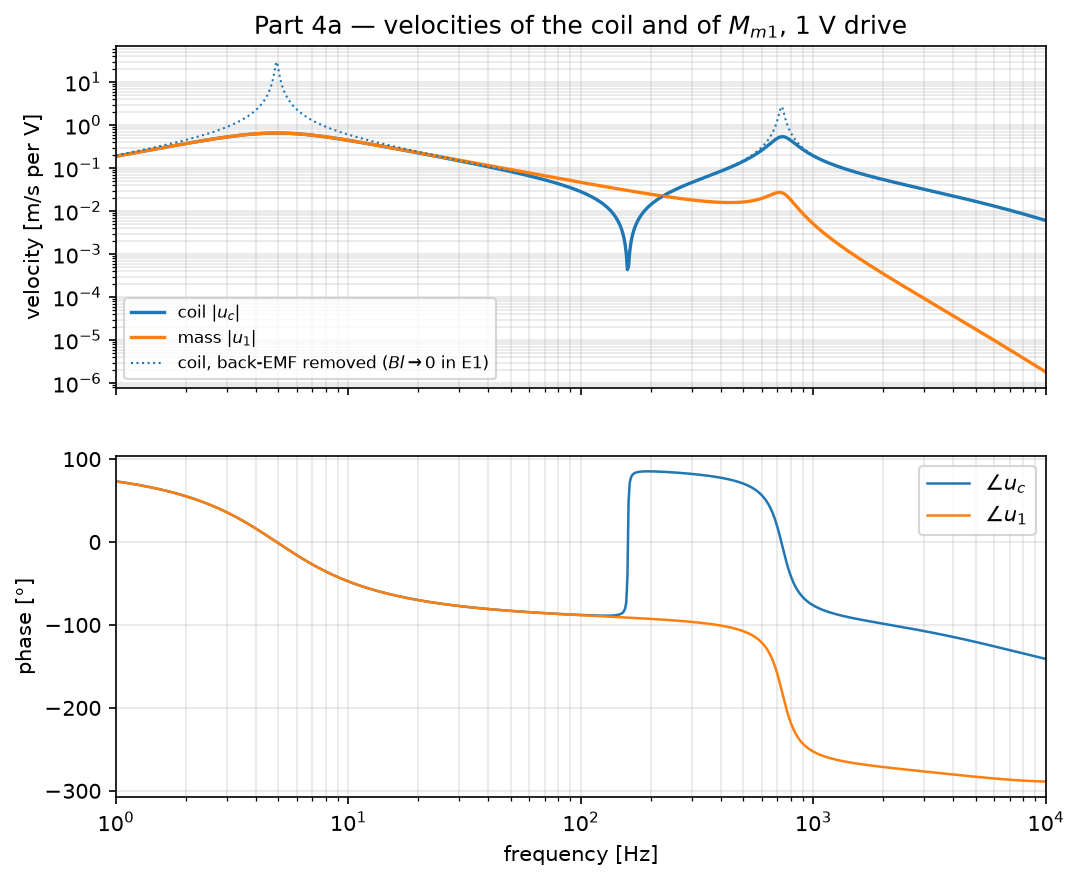
\includegraphics[width=0.85\linewidth]{part4a_velocities}
\caption{Part 4a: coil velocity $u_c$ and mass velocity $u_1$ per volt, magnitude and phase, \SIrange{1}{10000}{\hertz}; dotted: $u_c$ with the back-EMF removed.}
\label{fig:p4a}
\end{figure}

\emph{\SI{4.9}{\hertz}, rigid-body mode.} $C_{ms}$ (\SI{0.01}{\milli\metre\per\newton}) is a thousand times stiffer
than $C_{ms2}$, so at low frequency coil and mass move as one lump of \SI{105}{\gram} on the soft suspension
$C_{ms2}$ (hand: \SI{4.91}{\hertz}); both velocities are equal and in phase. The peak is broad because the electrical
damping of \SI{4.5}{\newton\second\per\metre} dominates ($Q\approx\omega_0M/R\approx0.7$); with the back-EMF removed
the same mode is damped only by $R_{ms2} = \SI{0.1}{\newton\second\per\metre}$ and peaks at
\SI{29.5}{\metre\per\second\per\volt}. Below the resonance the motion is compliance-controlled ($u\propto\jw$,
$+\SI{90}{\degree}$), between the resonances mass-controlled ($u\propto1/\jw$, \SI{-90}{\degree}).

\emph{\SI{158.5}{\hertz}, the coil stops.} This is the anti-resonance of the mechanical load: $M_{m1}$ on the stiff
spring $C_{ms}$ resonates ($1/(2\pi\sqrt{M_{m1}C_{ms}}) = \SI{159}{\hertz}$) and presents an almost infinite impedance
to the coil, so $u_c$ drops to \SI{4e-4}{\metre\per\second\per\volt} while $u_1$ keeps moving ($|u_1/u_c|$ about 40 right
at the dip). It is the tuned-mass-damper effect; the phase of $u_c$ jumps by \SI{180}{\degree} there.

\emph{\SI{733}{\hertz}, coil-on-spring mode.} The \SI{5}{\gram} coil bounces on $C_{ms}$ against the heavy, now almost
stationary mass (reduced-mass estimate \SI{729}{\hertz}). $u_c$ peaks at \SI{0.54}{\metre\per\second\per\volt};
$u_1$ shows only a small hump (0.027) and then falls at \SI{40}{\decibel} per decade because the spring cannot transmit
the force to $M_{m1}$ at high frequency (mass isolation). Above \SI{733}{\hertz} $u_c$ falls as $1/(\omega M_{mc})$,
and above \SI{8}{\kilo\hertz} $L_e$ also starts to limit the current. The shallow minimum of $u_1$ at \SI{436}{\hertz} is
a zero of its transfer function (the spring force and the $C_{ms2}/R_{ms2}$ branch partially cancel), not a system
resonance.

\FloatBarrier
\paragraph{b) Mechanical input impedance seen by the force (Fig.~\ref{fig:p4b}).} $Z_M = f/u_c = Bl\,I(V_{s1})/V(u_c)$
(KiCad expression \texttt{1.5*I(Vs1)/V(/u\_c)}).
\begin{table}[H]\centering\small
\begin{tabular}{@{}llll@{}}\toprule
Feature & $f$ & $|Z_M|$ [\si{\newton\second\per\metre}] & Phase \\ \midrule
\SI{1}{\hertz} & --- & 15.2 & \SI{-90}{\degree} ($C_{ms2}$ dominates) \\
\textbf{resonance (minimum)} & \SI{4.90}{\hertz} & 0.10 ($\approx R_{ms2}$) & \SI{0}{\degree} \\
\textbf{anti-resonance (maximum)} & \SI{158.5}{\hertz} & \num{6.9e3} & \SI{0}{\degree} (flip $+90\to-90$) \\
\textbf{resonance (minimum)} & \SI{732.8}{\hertz} & 1.13 ($\approx R_{ms}$) & \SI{0}{\degree} \\
\SI{10}{\kilo\hertz} & --- & $313\approx\omega M_{mc}$ & $+\SI{90}{\degree}$ (coil mass) \\
\bottomrule\end{tabular}
\caption{Part 4b extracted numbers.}
\end{table}
The impedance seen by the force is that of the pure mechanical network: the transducer is lossless, so $Z_M$ does
\emph{not} contain the electrical damping, which acts on the electrical side. Minima are where the force meets almost
no impedance, only the dampers, i.e.\ the two resonances; at \SI{4.9}{\hertz} $|Z_M|\approx R_{ms2}$ and at
\SI{733}{\hertz} $|Z_M|\approx R_{ms}$, so the damper values can be read straight off the plot. The maximum is the
anti-resonance where $M_{m1}$ on $C_{ms}$ takes all the force and the coil cannot move. The phase sequence
$-90/+90/-90/+90^\circ$ reads: compliance-like below \SI{4.9}{\hertz} ($C_{ms2}$), mass-like between 4.9 and
\SI{158}{\hertz} (the \SI{105}{\gram} lump), compliance-like between 158 and \SI{733}{\hertz} ($C_{ms}$, the coil is
spring-controlled), mass-like above ($M_{mc}$).

\begin{figure}[!htb]\centering
\begin{subfigure}{0.49\linewidth}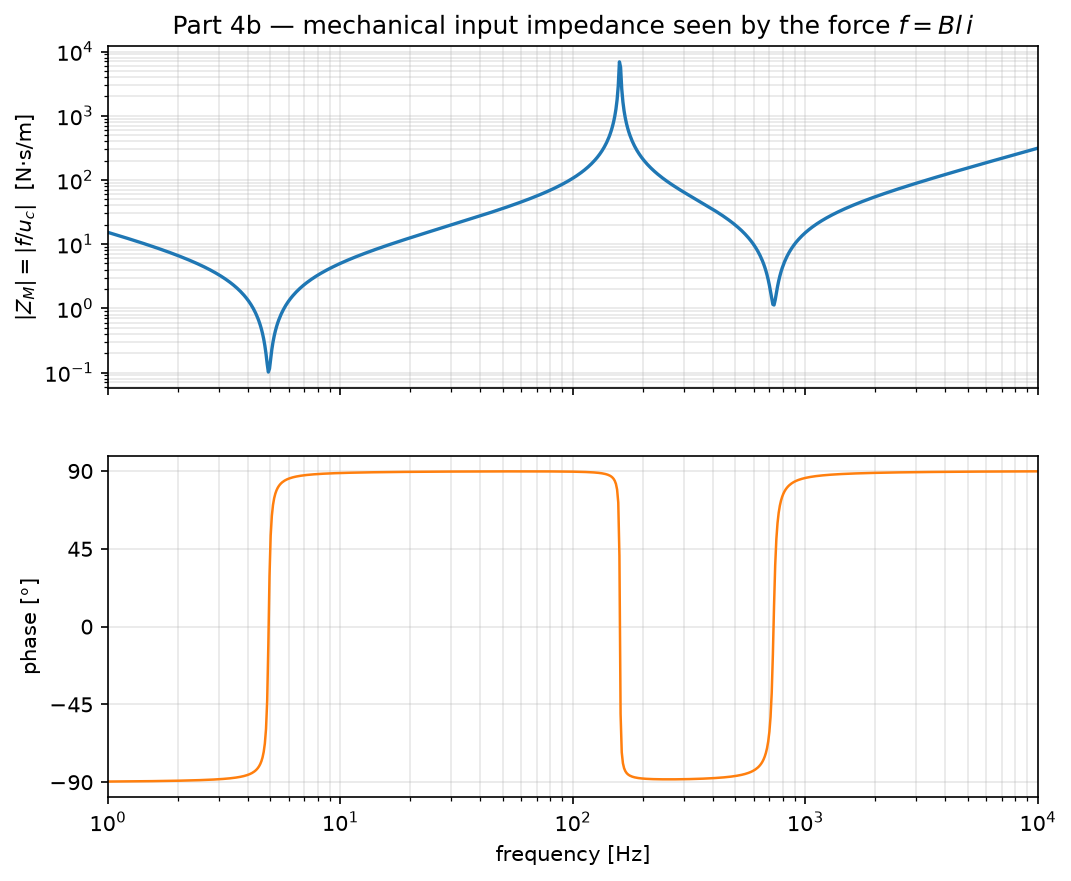
\includegraphics[width=\linewidth]{part4b_mechanical_impedance}\caption{$Z_M = Bl\,i/u_c$}\label{fig:p4b}\end{subfigure}
\begin{subfigure}{0.49\linewidth}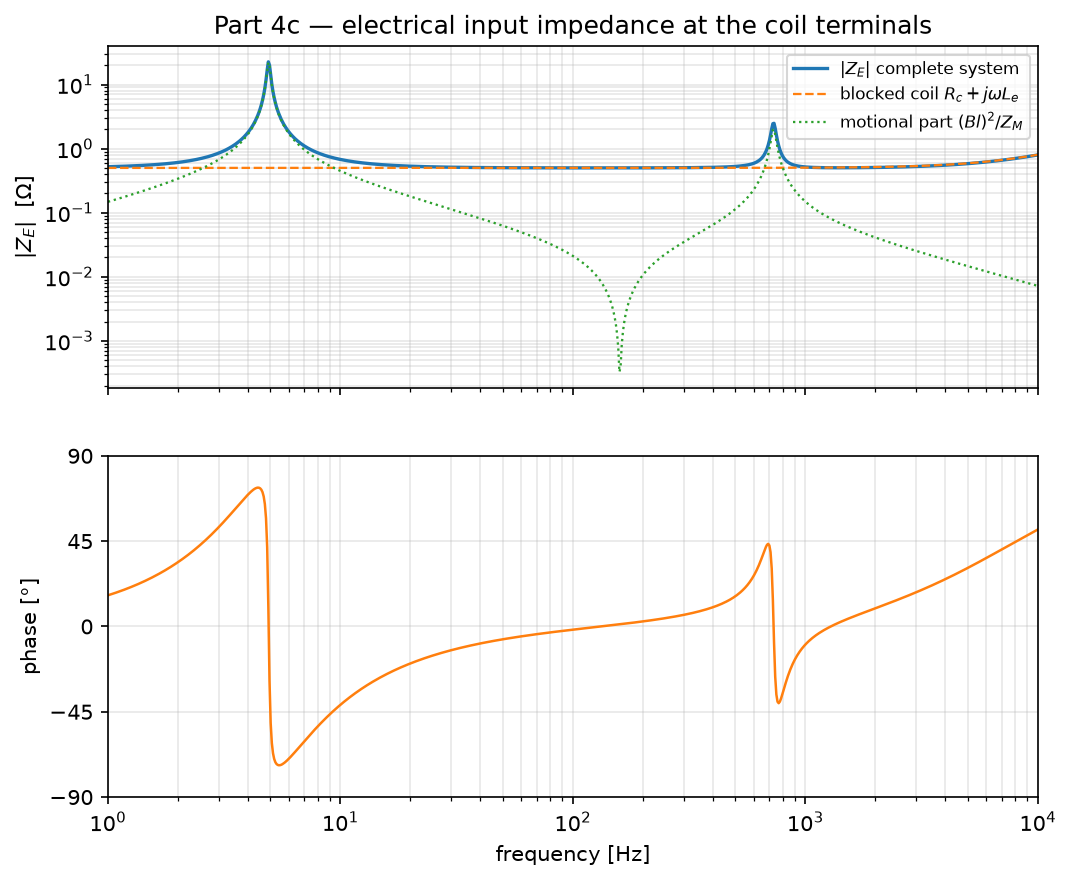
\includegraphics[width=\linewidth]{part4c_electrical_impedance}\caption{$Z_E = 1/I(V_{s1})$}\label{fig:p4c}\end{subfigure}
\caption{Part 4b/c: mechanical impedance seen by the electromagnetic force and electrical impedance seen by the
\SI{1}{\volt} source --- mirror images scaled by $(Bl)^2$.}
\end{figure}

\FloatBarrier
\paragraph{c) Electrical input impedance (Fig.~\ref{fig:p4c}).}
\begin{table}[H]\centering\small
\begin{tabular}{@{}lll@{}}\toprule
Feature & $f$ & $|Z_E|$ \\ \midrule
\SI{1}{\hertz} & --- & \SI{0.522}{\ohm} \\
\textbf{peak} & \SI{4.90}{\hertz} & \SI{22.6}{\ohm} (motional part \SI{22.1}{\ohm}) \\
broad minimum & 100--\SI{400}{\hertz} & \SI{0.500}{\ohm} $= R_c$ \\
\textbf{peak} & \SI{732.8}{\hertz} & \SI{2.48}{\ohm} (motional 1.98) \\
dip & \SI{1.4}{\kilo\hertz} & \SI{0.5025}{\ohm} \\
\SI{10}{\kilo\hertz} & --- & \SI{0.797}{\ohm} $\approx|R_c + \jw L_e| = 0.803$ \\
\bottomrule\end{tabular}
\caption{Part 4c extracted numbers.}
\end{table}
$Z_E = R_c + \jw L_e + (Bl)^2/Z_M$: the motional term is the \emph{inverse} of the mechanical impedance (Lecture 4A,
impedance conversion $Z_{E,M} = (Bl)^2Y_M$). So the mechanical \emph{resonances} ($Z_M$ minima) appear as \emph{peaks}
in $|Z_E|$, $(Bl)^2/R_{ms2} = \SI{22.5}{\ohm}$ at \SI{4.9}{\hertz} and $(Bl)^2/1.13 = \SI{2.0}{\ohm}$ at \SI{733}{\hertz}
on top of $R_c$, while the mechanical \emph{anti-resonance} (\SI{158}{\hertz}) is where $Z_E$ is closest to $R_c$
($(Bl)^2/\num{6.9e3} = \SI{0.3}{\milli\ohm}$): the coil is blocked, there is no back-EMF, and the electrical side sees the
blocked-coil impedance. The $Z_E$ peaks are sharp because on the electrical side the mechanical resonance is loaded only
by the mechanical dampers ($Q\approx 2\pi\cdot4.9\cdot0.105/0.1\approx32$ for the first mode). The phase of $Z_E$ swings
about $\pm\SI{75}{\degree}$ around the peaks (inductive below a resonance, capacitive above): a motional impedance looks
like a parallel RLC on the electrical side, the classic loudspeaker impedance curve. Above about \SI{1.4}{\kilo\hertz} the
motional term is negligible and $Z_E$ follows $R_c + \jw L_e$ with its corner at \SI{8}{\kilo\hertz}
($+\SI{47}{\degree}$, \SI{0.8}{\ohm} at \SI{10}{\kilo\hertz}). Compared with b), $Z_M$ and $Z_E$ are mirror images on a
log scale, every minimum of one a maximum of the other, scaled by $(Bl)^2 = 2.25$.

\FloatBarrier
\paragraph{d) Every resonance and anti-resonance (Fig.~\ref{fig:p4all}).}
\begin{table}[H]\centering\small
\begin{tabular}{@{}p{1.2cm}p{2.0cm}p{1.8cm}p{2.1cm}p{2.0cm}p{4.9cm}@{}}\toprule
$f$ & $u_c$ & $u_1$ & $Z_M$ & $Z_E$ & Physical origin \\ \midrule
\SI{4.9}{\hertz} & peak 0.65 & peak 0.65 & min 0.10 ($\approx R_{ms2}$) & peak \SI{22.6}{\ohm} & both masses (\SI{105}{\gram}) on the soft suspension $C_{ms2}$; rigid-body mode, damped mostly by $(Bl)^2/R_c$ \\
\SI{158.5}{\hertz} & \textbf{dip} \num{4e-4} (coil stands still) & still moving & \textbf{max} \num{6.9e3} & $\approx R_c$ & $M_{m1}$ resonating on the stiff spring $C_{ms}$ absorbs the force: anti-resonance, tuned-mass-damper effect \\
\SI{436}{\hertz} & --- & shallow dip & --- & --- & zero of the $u_1$ transfer function (spring force vs.\ suspension branch), not a system mode \\
\SI{733}{\hertz} & peak 0.54 & small hump 0.027 & min 1.13 ($\approx R_{ms}$) & peak \SI{2.5}{\ohm} & coil (\SI{5}{\gram}) bouncing on $C_{ms}$ against the nearly stationary $M_{m1}$ (reduced mass \SI{4.76}{\gram}, \SI{729}{\hertz}) \\
\SI{8}{\kilo\hertz} & roll-off steepens & --- & --- & inductive rise & electrical corner $R_c/(2\pi L_e)$; $L_e$ limits the current, no mechanical origin \\
\bottomrule\end{tabular}
\caption{Part 4d: all features of the three plots and their origin.}
\end{table}
Forces as a function of the driving current: the coil force is always $f = Bl\,i$; the force in the spring $C_{ms}$ is
$f - \jw M_{mc}u_c$, which is $\approx f$ below \SI{158}{\hertz} (the coil mass is negligible) and tends to zero above
\SI{733}{\hertz}, where the coil mass takes the whole force.

\begin{figure}[!htb]\centering
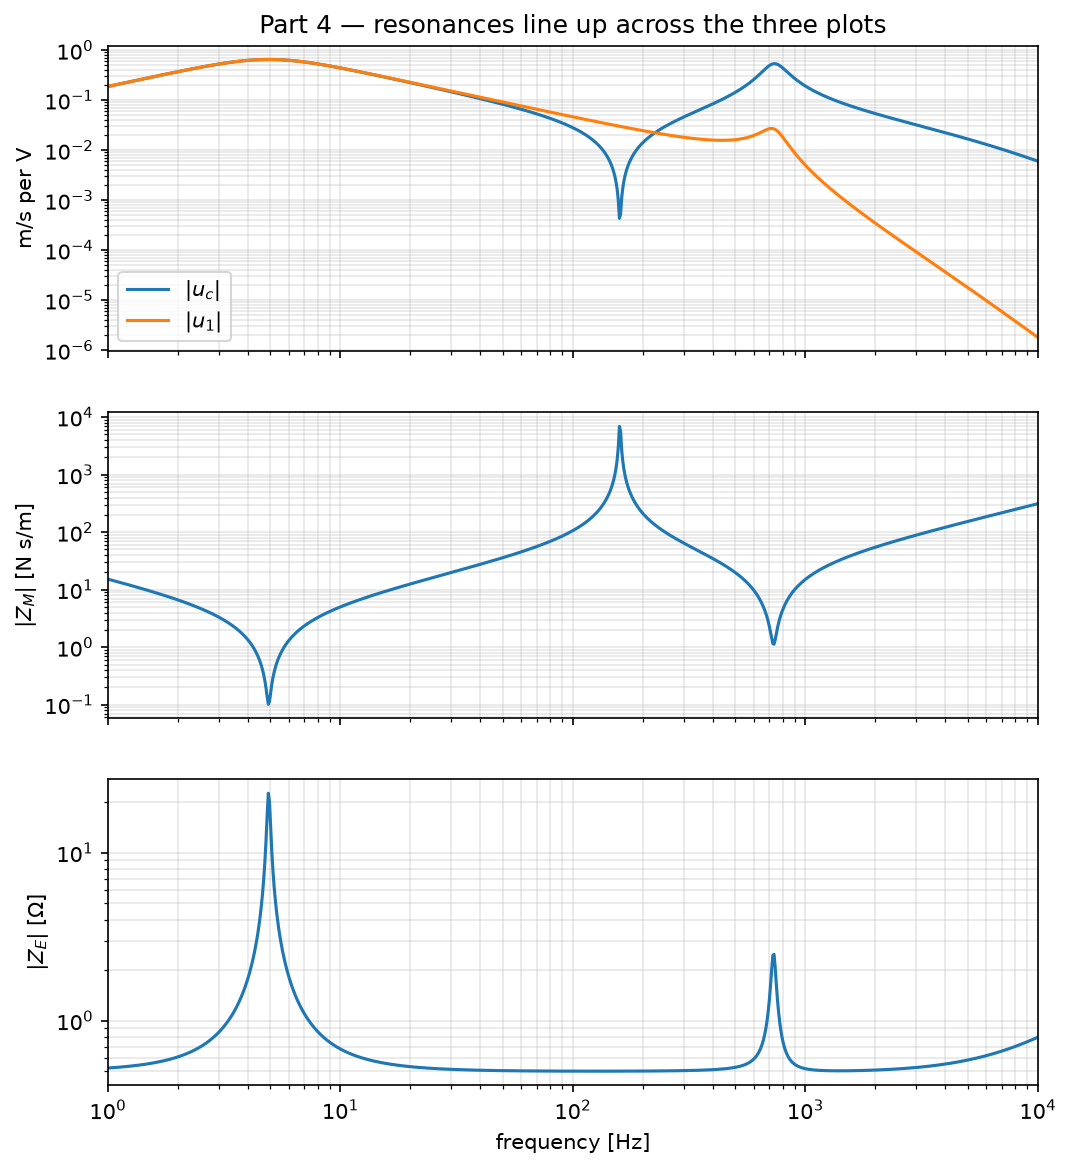
\includegraphics[width=0.62\linewidth]{part4_overview}
\caption{Part 4d: velocities, $Z_M$ and $Z_E$ on one frequency axis; every resonance of one plot lines up with an anti-resonance of another.}
\label{fig:p4all}
\end{figure}

\FloatBarrier
\paragraph{Modelling choices and validity.} The mobility analogy was used for the mechanical side; in the impedance
analogy the same circuit needs a gyrator (H/F sources) instead of the G/E pair, and the plots are identical. The coil
current is sensed as the voltage across $R_c$ (gain $Bl/R_c$), which is exact for a linear resistor. Frequencies are
read from a 200-points-per-decade sweep, accurate to about \SI{0.5}{\percent}.


%% ======================================================================
\FloatBarrier
\section{Conclusion}
The four systems reduce to the same two ideas. First, an electromechanoacoustic system is an RLC network once the
analogy is chosen consistently: in the mobility analogy every mass is a capacitor to ground and every spring an
inductor, in the acoustic impedance analogy every closed volume is a grounded capacitor and every narrow tube an
inductor with its loss in series. Second, a transducer is a pair of controlled sources with a constant gain ($S$ or
$Bl$), and everything on the far side of it is seen through that gain: an acoustic load becomes $S^2Z_A$ on the
mechanical side, a mechanical impedance becomes $(Bl)^2/Z_M$ on the electrical side, which is why mechanical
resonances show up as peaks in the electrical impedance.

The simulations reproduced every hand estimate: the \SI{51}{\hertz} single-mass resonance and the \SI{1.3}{\kilo\hertz}
absorber of the Lowther dual cone (Part 1); the ladder resonances of the silencer and the fact that a pressure
source and a volume-velocity source excite complementary sets of natural frequencies (Part 2); the \SI{4}{\gram} of
air mass and the \SI{22}{\newton\second\per\metre} of radiation resistance the baffle adds to the two cones (Part 3);
the \SI{4.9}{\hertz} and \SI{733}{\hertz} modes of the coil system and their mirror image in $Z_E$ (Part 4). The
most instructive results are the ones the circuit gives for free: the mechanical crossover of the dual diaphragm,
whose far-field response stays flat to \SI{10}{\kilo\hertz} at the cost of \SI{13}{\decibel} once only the inner
cone radiates; the silencer amplifying the exhaust by \SI{26}{\decibel} at its resonances while attenuating
\SI{110}{\decibel} at \SI{1}{\kilo\hertz}, of which the upper half is outside the validity of the lumped model; and
the sign of the back-EMF, which is easy to get wrong and immediately visible as a \SI{45}{$\times$} change in the
velocity peak.

%% ======================================================================
\FloatBarrier
\section*{Appendix A: reproducing the simulations}
Everything lives in \texttt{5.~Semester/Electroacoustics/Labs/Lab A/}:
\begin{itemize}[nosep]
\item \texttt{KiCad/} holds one project per sheet (Table~\ref{tab:projects}), each a full KiCad~10 project:
      \texttt{.kicad\_pro}, \texttt{.kicad\_sch} with the \texttt{.ac} directive as sheet text, \texttt{.wbk} workbook
      with the traces preloaded, and the exported \texttt{.cir}. Open the schematic and run \emph{Inspect $\to$ Simulator}.
\item \texttt{sim/part1.py} to \texttt{part4.py} --- standalone scripts that draw the sheets (\texttt{schdraw}),
      export the netlist, run ngspice in batch, post-process with numpy and write the figures; helper modules alongside.
\item \texttt{results/partN.md} --- element tables, all extracted numbers and the interpretation behind this report.
\end{itemize}
\begin{table}[H]\centering\small
\begin{tabular}{@{}lll@{}}\toprule
Project folder & Part & Drive / variant \\ \midrule
\texttt{Part1\_DualDiaphragm\_Stiff} & 1 & \SI{1}{\newton}, $C_{md} = \SI{e-10}{\metre\per\newton}$ \\
\texttt{Part1\_DualDiaphragm\_Soft} & 1 & \SI{1}{\newton}, $C_{md} = \SI{3e-6}{\metre\per\newton}$ \\
\texttt{Part2a\_Silencer\_PressureSource} & 2a & \SI{1}{\pascal}, ideal open end \\
\texttt{Part2b\_Silencer\_VolumeVelocitySource} & 2b, 2c & \SI{1}{\cubic\metre\per\second}, ideal open end \\
\texttt{Part2d\_Silencer\_Radiation} & 2d, 2e & \SI{1}{\cubic\metre\per\second}, radiation network \\
\texttt{Part3\_Coupled\_Stiff} / \texttt{\_Soft} & 3 & Part 1 + radiation on both diaphragms \\
\texttt{Part4\_Coil\_Electromechanical} & 4 & \SI{1}{\volt} \\
\bottomrule\end{tabular}
\caption{KiCad projects.}\label{tab:projects}
\end{table}
The batch path used by the scripts is
\begin{verbatim}
kicad-cli sch export netlist --format spice -o X.cir X.kicad_sch
ngspice -b run.cir
# run.cir:  .include X.cir
#           .control
#           run
#           wrdata out.txt v(/node) i(Vs1) ...
#           .endc
\end{verbatim}
and \texttt{wrdata} writes frequency, real and imaginary part per vector.

\paragraph{Translation to LTspice for the quiz.} The circuits are tool-agnostic. KiCad's \texttt{GSOURCE} (VCCS) is
LTspice's \texttt{G} and \texttt{ESOURCE} (VCVS) is \texttt{E}; the SPICE line is identical
(\texttt{G1 N+ N- C+ C- gain}, current flows from N+ through the source to N-). A \SI{0}{\volt} voltage source in
series with a branch gives its current as \texttt{I(Vs)} in both tools. The mobility-analogy impedance trick is the same:
drive with a \SI{1}{\ampere} current source and plot \texttt{1/V(u)}; in LTspice use \emph{Add traces} with the
expression, in KiCad a user-defined signal. Every node needs a DC path to ground, so a current source feeding a
capacitor-only branch gets a \SI{100}{\mega\ohm} leak.

\FloatBarrier
\section*{Appendix B: KiCad schematics}
\begin{figure}[H]\centering
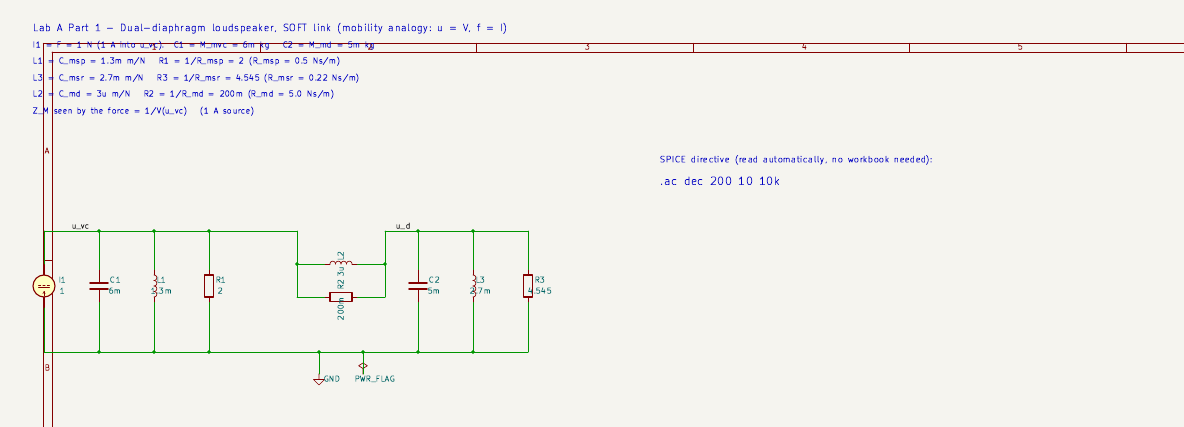
\includegraphics[width=0.95\linewidth]{sch_crop_Part1_DualDiaphragm_Soft}
\caption{Part 1, soft link (the stiff sheet differs only in $L_2$ and $R_2$).}
\end{figure}
\begin{figure}[H]\centering
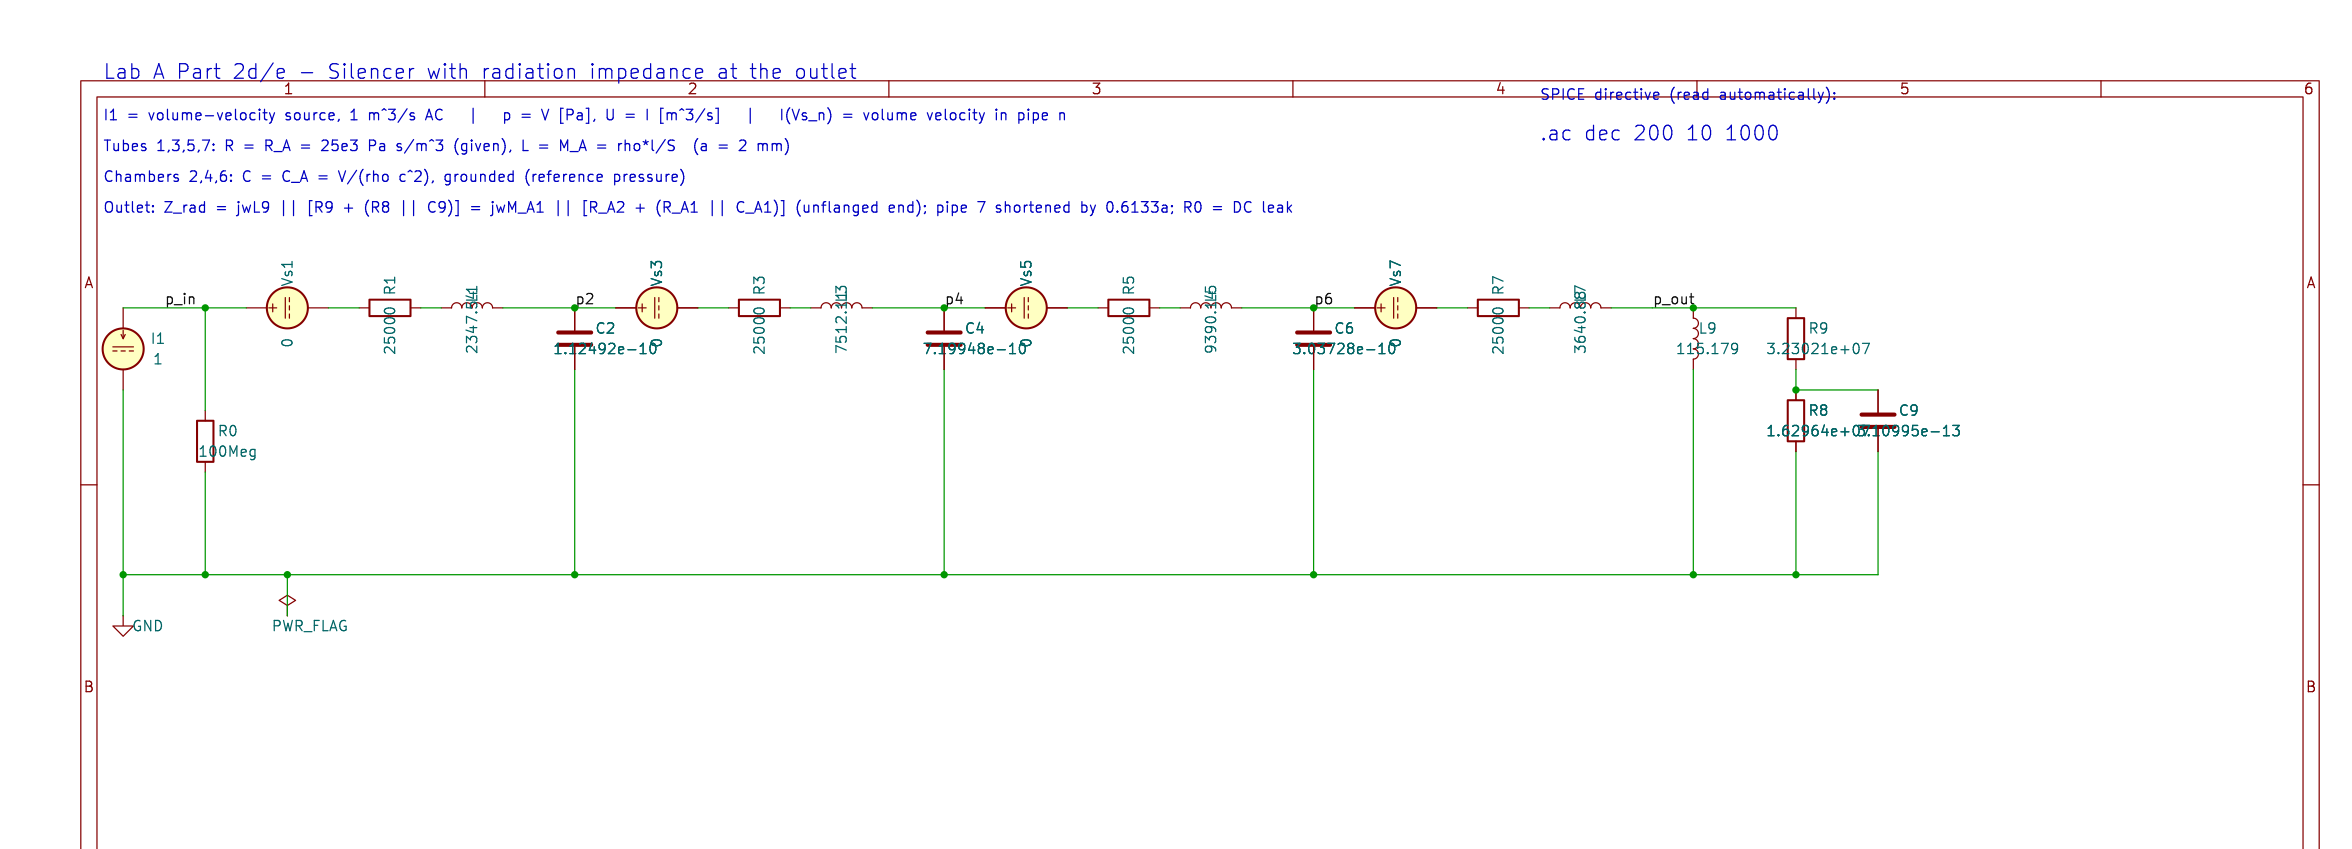
\includegraphics[width=\linewidth]{sch_crop_Part2d_Silencer_Radiation}
\caption{Part 2d: silencer with the radiation network at the outlet (sheets 2a/2b are the same ladder with an ideal open end and a pressure or volume-velocity source).}
\end{figure}
\begin{figure}[H]\centering
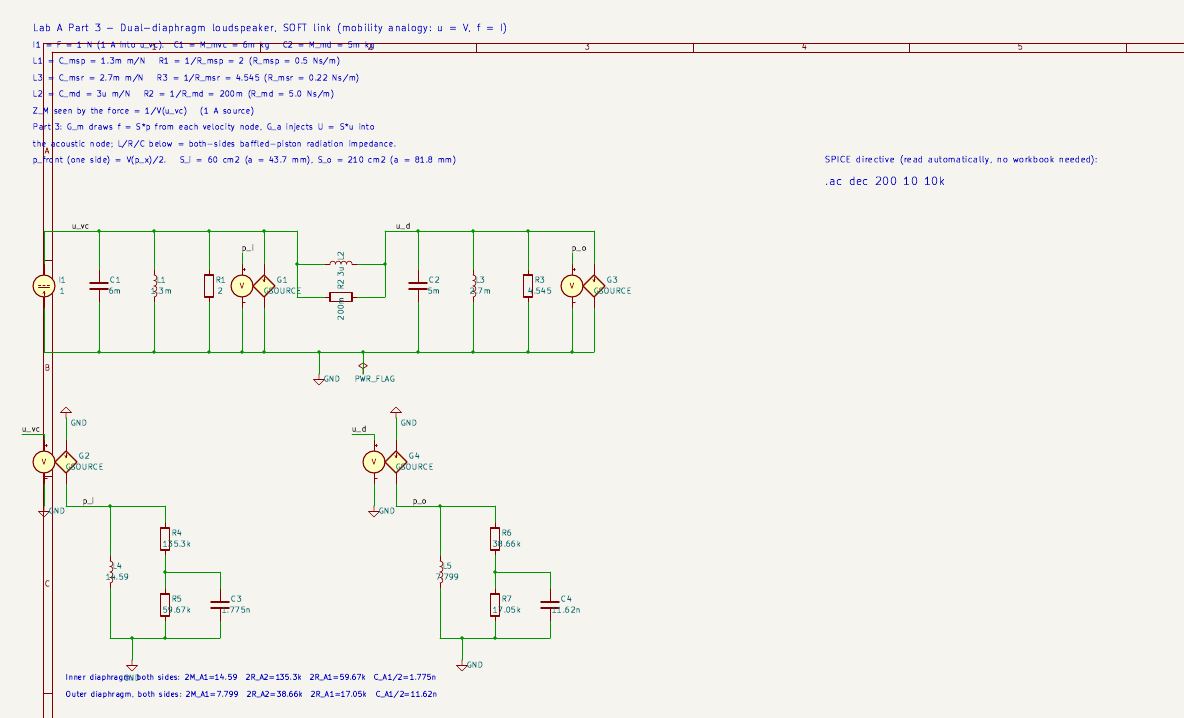
\includegraphics[width=0.9\linewidth]{sch_crop_Part3_Coupled_Soft}
\caption{Part 3, soft link: the Part 1 network with two radiation sub-networks coupled by G-sources.}
\end{figure}
\begin{figure}[H]\centering
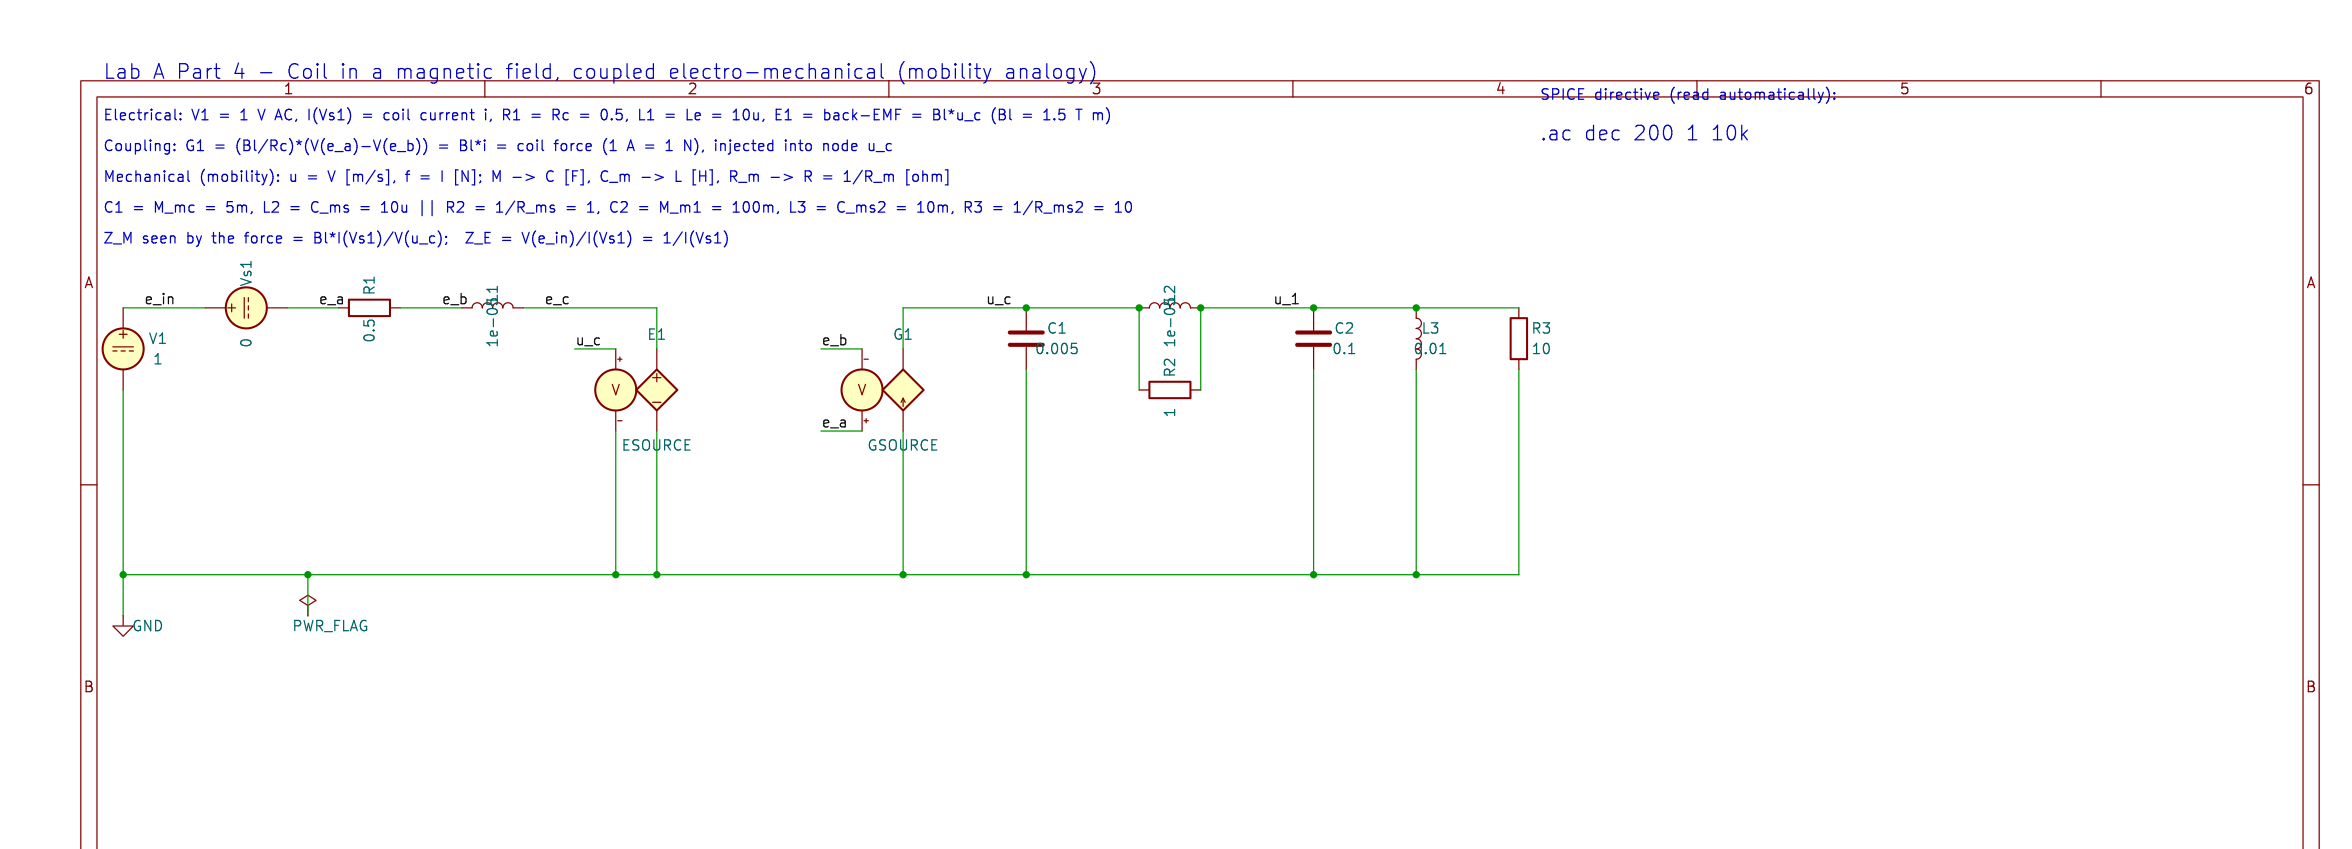
\includegraphics[width=\linewidth]{sch_crop_Part4_Coil_Electromechanical}
\caption{Part 4: electrical loop with back-EMF VCVS, force VCCS into the mobility network.}
\end{figure}

\end{document}
